%%%%%%%%%%%%%%%%%%%%%%%%%%%%%%%%%%%%%%%%%%%%%%%%%%%%%%%%%%%%%%%%%%%%%%%%%%%%%%%
%%% Describe the results of the NINJA-2 mock data challenge.
%%%%%%%%%%%%%%%%%%%%%%%%%%%%%%%%%%%%%%%%%%%%%%%%%%%%%%%%%%%%%%%%%%%%%%%%%%%%%%%

\newcommand{\roughly}{\mathchar"5218\relax}
\newcommand{\Answer}[1]{\blue{[#1]}}

% \normalem

\newcommand{\Ys}{{{}^{-s}Y}}
\newcommand{\Ytwo}{{{}^{-2}Y}}
\newcommand{\lie}{\mathcal{L}}
\newcommand{\vek}[1]{\boldsymbol{#1}}
\newcommand{\vdag}{(v)^\dagger}
\newcommand{\ihope}{\texttt{ihope}}
\newcommand{\subrows}[2][c]{%
  \begin{tabular}[#1]{@{}c@{}}#2\end{tabular}}
\def\no{\nonumber \\}
\def\nn{\nonumber}
\def\ver{\vskip 12pt}
\def\lll{\left[}
\def\rrr{\right]}
\def\bl{\Biggl[}
\def\br{\Biggr]}
\def\gbl{\Biggl\{}
\def\gbr{\Biggr\}}

\newcommand{\define}{\colonequals}
\newcommand{\eob}{\texttt{EOBNRv2}\xspace}
\newcommand{\imr}{\texttt{PhenomB}\xspace}
\newcommand{\imrns}{\texttt{PhenomB$_\mathtt{\chi=0}$}\xspace}

\def\lm{{\ell m}}
\def\ii{{\rmi}}
\def\o{\omega}
\def\IL{\relax{\rm I\kern-.18em L}}
\def\tT{{\tilde T}}

\newcommand{\pstar}{{p^*}}
\newcommand{\bstar}{{b^*}}
\newcommand{\bbar}{{\bar{b}}}
\newcommand{\Ebar}{{\bar{E_r}}}
\newcommand{\kstar}{{k^*}}
\newcommand{\Screll}{{\mathcal{L}}}
\newcommand{\Scri}{{\mathcal{I}}}
\def\rg{\sqrt{-g}}

\newcommand{\Mc}{\ensuremath{\mathcal{M}}}
\newcommand{\Ms}{\ensuremath{\mathrm{M}_{\odot}}}
% \newcommand{\msun}{\ensuremath{\mathrm{M}_\odot}}

\newcommand{\Overlap}[1]{\Olap\left( #1 \right)}

\def\CQG{\textit{Class.~Quantum Grav.~}}
\def\PRD{\textit{Phys.~Rev.~D}}

\newcommand{\m}{\langle}
% \newcommand{\M}{\rangle}

\def\ltsima{$\; \buildrel < \over \sim \;$}
\def\simlt{\lower.5ex\hbox{\ltsima}}
\def\gtsima{$\; \buildrel > \over \sim \;$}
\def\simgt{\lower.5ex\hbox{\gtsima}}

\makeatletter
\let\protect\relax
{\catcode`\|=\active
  \xdef\InnerProduct{\protect\expandafter\noexpand\csname InnerProduct
\endcsname}
  \expandafter\gdef\csname InnerProduct \endcsname#1{%
    \begingroup
    \ifx\SavedDoubleVert\relax
    \let\SavedDoubleVert\|\let\|\IpDoubleVert
    \fi
    \mathcode`\|32768\let|\IPVert
    \left({#1}\right)
    \endgroup
  }
}
\def\IPVert{\@ifnextchar|{\|\@gobble}% turn || into \|
     {\egroup\,\mid@vertical\,\bgroup}}
\def\IPDoubleVert{\egroup\,\mid@dblvertical\,\bgroup}
\let\SavedDoubleVert\relax
\def\midvert{\egroup\mid\bgroup}
\def\SetVert{\@ifnextchar|{\|\@gobble}% turn || into \|
    {\egroup\;\mid@vertical\;\bgroup}}
\def\SetDoubleVert{\egroup\;\mid@dblvertical\;\bgroup}
\def\mid@vertical{\mskip1mu\vrule\mskip1mu}
\def\mid@dblvertical{\mskip1mu\vrule\mskip2.5mu\vrule\mskip1mu}


% \section{Introduction}
% \label{sec:introduction}
% A network of second-generation laser interferometric
% gravitational-wave (GW) observatories is presently under construction.
% The US-based Advanced Laser Interferometer Gravitational Wave 
% Observatory (aLIGO)~\cite{Harry:2010zz} is expected to have its
% initial observing run in 2015 utilizing observatories in Hanford,
% Washington and Livingston, Louisiana (denoted ``H'' and ``L'', respectively). 
% aLIGO will then work towards reaching design
% sensitivity, expected in 2018-20~\cite{Aasi:2013wya}. The
% French-Italian Advanced Virgo (AdV) observatory~\cite{Accadia:2011zzc,aVIRGO}
% (denoted ``V'') is expected to follow shortly after the
% aLIGO instruments. The cryogenically cooled KAGRA
% observatory~\cite{Kuroda:2010zzb,Somiya:2011np} and a India-based aLIGO
% facility~\cite{LIGODCC:M1100296,Unnikrishnan:2013qwa} are due to begin 
% operations around
% 2020, providing a 5-site network to explore the gravitational-wave sky
% in detail.
% 
% These second-generation observatories will have an order of magnitude
% increase in sensitivity over their first generation counterparts and
% will be sensitive to a broader range of gravitational-wave
% frequencies~\cite{Harry:2010zz,aVIRGO,Somiya:2011np}. One of the
% primary observational targets for this global network is the inspiral, merger 
% and ringdown of a binary system containing two black 
% holes~\cite{thorne.k:1987}. 
% With aLIGO and AdV operating at their final design sensitivities
% it is expected that 0.4 - 1000 binary black hole (BBH) coalescences
% will be observed per year of operation~\cite{Abadie:2010cf}.  Directly
% observing the collision of two black holes will allow
% gravitational-wave astronomers to understand the physics of black-hole
% spacetimes and to explore the strong-field conditions of the
% theory of general relativity~\cite{Sathyaprakash:2009xs}.

% Exploring the underlying mass and spin distributions of stellar-mass black
% holes can tell us a great deal about the end stages of massive-star evolution.
% The mass measurements of compact objects made to date suggest a gap between the
% most massive neutron stars ($\lesssim 3~\msun$)~\cite{Kalogera:1996ci} and the
% least massive black holes ($\gtrsim 5~\msun$)~\cite{Bailyn:1997xt}.  It is
% still an open question as to whether this gap is real and the result of
% formation mechanisms, or simply due to observational biases~\cite{Farr:2010tu}.
% Whether or not ground-based detectors will be able to distinguish between
% these regions in mass space is of great interest. Furthermore, from the
% distributions of black hole spin magnitudes and tilts (orientation of the spin
% relative to the orbital angular momentum), more can be learned about supernovae
% kicks and compact binary formation environments.  Stellar-mass black hole spin
% measurements are currently done by modelling either the accretion disk's thermal
% continuum X-ray spectrum, or the profile of the broadened Fe K$\alpha$
% line~\cite{McClintock:2011zq}.  Both methods are fundamentally based on
% assumptions about the location of the inner edge of the accretion disk, and
% also depend sensitively on very complicated physical models of the disk and its
% emission.  Gravitational waves will provide an entirely new method of
% measuring black hole spin which does not require the complicated modeling of
% accretion disk physics. 

Of the stellar mass black hole angular momenta (spin) measurements made to 
date, half are found to have a magnitude
$a=|\vec{S}|/M^2|\gtrsim0.8$~\cite{McClintock:2011zq}. With BBH observations, aLIGO and AdV 
will be able to provide independent measurements of the black hole spin 
magnitudes. Therefore, it will be interesting
to evaluate how well aLIGO and Advanced Virgo (AdV)
will be able to constrain the magnitude of 
the black holes' component spins.
The direction of the compact objects' angular momenta is also
of interest, with particular implications for formation
mechanisms~\cite{Belczynski:2007xg}.  Measuring systems with component
spins misaligned with the orbital angular momentum is outside of the
scope of this project. However, this study does include systems with
component spins that are both aligned and anti-aligned with the
orbital angular momenta, and we will evaluate the ability of aLIGO and AdV to
distinguish such systems from one another.
% 
% The standard technique for observing BBH mergers
% involves matched-filtering data taken from gravitational-wave observatories 
% against ``template'' waveforms that should closely match potential 
% astrophysical signals~\cite{Wainstein:1962,Wainstein:1968,Allen:2005fk}. The
% observable BBH waveform includes the signal from the inspiral of the
% two black holes, as well as their merger and the resulting black
% hole's ringdown. Search templates must include all of these
% features~\cite{Buonanno:2009zt,Brown:2012nn}.  As an alternative to
% matched-filter searches, a number of algorithms exist to perform
% searches for \emph{unmodelled} gravitational-wave signals
% \cite{Klimenko:2008fu,Searle:2007uv,Sutton:2009gi}. These algorithms
% do not require accurate knowledge of the waveforms to make
% observations, but are not as sensitive as matched-filter searches in
% cases where the waveform models are well understood.
% 
% Theoretical models of the inspiral, merger and ringdown of BBH systems
% are necessary to produce template banks for matched-filter searches
% and to use as model signals to test both matched-filter and unmodelled
% searches.  The inspiral portion of the waveform can be modeled by
% analytic post-Newtonian (PN) calculations
% \cite{Blanchet:2006zz,Buonanno:2009zt}, while numerical solutions of
% the General Relativity field equations are required to accurately
% model the final orbits and merger.  Prior to breakthroughs in
% numerical relativity (NR) in
% 2005~\cite{Pretorius2005,Campanelli:2005dd, Baker:2005vv}, template
% banks and search pipeline tests used only inspiral waveforms.  
Since
2007, NR waveforms have been used to calibrate analytical waveform
models~\cite{Buonanno:2007pf,Damour:2009kr,Pan:2011gk,Taracchini:2012ig,
Ajith:2009bn,Santamaria:2010yb,Damour:2012ky,Taracchini:2013rva}. Some
of the analytical waveforms have been already employed in search
pipelines~\cite{Aasi:2012rja}.  However, there exists another
useful and valuable avenue of communication between numerical
relativists and gravitational-wave astronomers.  As NR pushes into new
regions of parameter space the waveforms can be used directly to test
searches employing previously-calibrated templates, and the degree to
which these searches prove to be insufficient can motivate both new
template models and additional simulations.

The Numerical INJection Analysis (NINJA) project was created in 2008. 
The project uses recent 
advances in numerical relativity~(\cite{Centrella:2010mx} and references
therein) to test analysis 
pipelines by adding numerically-modelled, physically-realistic signals to 
detector noise and attempting to recover these signals with search pipelines.
The first NINJA project (NINJA-1)~\cite{Aylott:2009ya} utilized a total of
23 numerical waveforms, which were injected into Gaussian noise colored with
the frequency sensitivity of initial LIGO and Virgo. These data were
analyzed by nine data-analysis groups using both search and
parameter-estimation algorithms~\cite{Aylott:2009ya}.  

However, there were four limitations to
the NINJA-1 analysis. First, due to the computational cost of NR simulations, 
most waveforms 
included only $\sim$10 orbits before merger. Therefore the waveforms were 
too short to inject over an astrophysically
interesting mass range without introducing artifacts into the data. The lowest
mass binary considered in NINJA-1 had a total mass of 35$\Ms$, whereas
the mass of black holes could extend below
$5\Ms$~\cite{Farr:2010tu,Ozel:2010su}.
Second, the waveforms were only inspected for obvious,
pathological errors and no cross-checks were performed between the
submitted waveforms. It was therefore difficult to assess the
physical fidelity of the results.  
Third, the NINJA-1 data set
contained stationary noise with the simulated signals already injected
into the data. Since the data set lacked the non-Gaussian noise transients 
present 
in real detector data, it was not possible to fully explore the response of the
algorithms in a real search scenario. Finally, the data set contained only 126 
simulated signals,
this precluded detailed statistical studies of the effectiveness of
search and parameter estimation algorithms. Despite these limitations,
the NINJA-1 project led to a framework within which to perform injection 
studies using waveforms as calculated by the full nonlinear general theory of 
relativity, established guidelines for such studies (in particular a 
well-defined format
for the exchange of NR waveforms~\cite{Brown:2007jx}), and clarified where 
further work was needed.

This lead to the initiation of the second NINJA project (NINJA-2), whose goals 
were to build and improve upon NINJA-1 and perform a systematic test of the 
efficiency of data-analysis pipelines in preparation for the Advanced detector 
era. A set of 60 NR waveforms were submitted by 8 numerical relativity groups 
for the NINJA-2 project~\cite{Ajith:2012az}. These waveforms conform 
to a set of length and accuracy requirements, and
are attached to PN inspiral signals to produce hybrid PN-NR waveforms that can 
be injected over the full range of physically relevant total binary masses.
The construction and verification of these waveforms is described 
in~\cite{Ajith:2012az}, and summarized here in 
section~\ref{sec:waveforms}.
% In the Numerical-Relativity and 
% Analytical-Relativity collaboration, a project complementary to the NINJA 
% collaboration, 22 new NR waveforms were produced and rigorously analysed. These 
% newly produced NR waveforms were compared to the most recent calibrated 
% analytical models, finding that the loss of event rates due to modeling is 
% below 3\%~\cite{Hinder:2013oqa}. 

In this chapter we study the ability of a search algorithm (called 
``\ihope{}'') that was 
used in the last of the Initial LIGO and Virgo science runs to observe
numerically-modelled BBH waveforms from the set %of 60 waveforms
submitted to the NINJA-2 project. 
% 
% There are a wide range of search and parameter estimation algorithms available
% within the GW astronomy community: those that were used in past analyses of
% detector data, old algorithms that have been updated and re-tuned following the
% experience gained in those analyses, plus many new algorithms under
% development.
The \ihope{} search pipeline is under constant development and re-tuning.
For both practical reasons, and to mark a clear point in the
development and refinement of the methods, we employed \emph{only} the
search methods that were approved and used in the
last initial-LIGO and Virgo science runs, \emph{without any additional tuning
or 
modifications}~\cite{Babak:2012zx,Aasi:2012rja,Abadie:2012rq}. 
By doing this we aim to provide a benchmark against which
future algorithms can be compared.
The data set used was obtained by recoloring actual detector data 
taken during LIGO's sixth and Virgo's second science runs to 
the sensitivity expected during the early science runs of Advanced LIGO
and Virgo.


A set of 7 numerical relativity waveforms, with
masses ranging from 14.4$M_{\odot}$ to 124$M_{\odot}$ were added into
the recolored data as an unbiased test of the process through which candidate 
events are identified for BBH waveforms. This 
data was distributed to analysts who
knew that such ``blind injections'' were present but had no
information about the number, parameters or temporal location of these
waveforms. 
% This was similar to blind injection tests conducted by the
% LIGO and Virgo collaborations in their latest science runs
% \cite{Colaboration:2011np}. Using a search for unmodelled gravitational wave 
% transients we found that one of these signals was recovered, with an estimated 
% false alarm rate of 1 every 47 years. The
% remaining 6 signals were consistent with background.
Two independent \ihope{} analysis were performed over the data.
One focused on {\it low}-mass binaries with 
$2M_\odot\leq m_1+m_2\leq 25M_\odot$, and the other on {\it high}-mass
binaries with $25<_\odot\leq m_1+m_2\leq 100M_\odot$.
Between the two analyses, 6 of the injected 
signals were recovered with more significance than all background
events. This allowed upper limits on the false alarm rate ranging
between 1 every 5800 years and 1 every 31000 years to be placed on
each blind injection. The remaining signal was not recovered due to
having a low network signal-to-noise ratio and possessing a large
anti-aligned spin, which was not modelled in the bank of waveforms used in the 
search.
% 
% Parameter estimation algorithms have come a long way since the first NINJA
% project. Previously these analyses were unable to estimate the parameters of
% high mass systems accurately due to the use of inspiral-only models on data
% with little measurable inspiral. We show that these tools are now capable of
% reliably providing parameter estimates for both low and high mass systems.
% For all but one injection the masses and spins of the black holes were recovered
% within the estimated 95\% credible regions.  The remaining injection suffered
% small systematic biases due to non-Gaussian features present in the noise, the
% modeling of which is an ongoing endeavor.
% We find that strong intrinsic degeneracies between the masses and black hole 
% spins \cite{Baird:2012cu,Hannam:2013uu} make it difficult to constrain the 
% masses well, for 3 of the signals the 
% presence of a neutron star cannot be ruled out. We also investigate the ability 
% to constrain the sky localization of the various signals and demonstrate how 
% even low power non-Gaussian noise transients in the data can effect the 
% recovery of the intrinsic parameters of BBH systems.
% 
% We use large sets of known waveforms to assess the 
% efficiency of the matched-filter BBH search algorithm as a 
% function of the mass and angular momenta of the component black holes. 
% These are the first such studies that have been done using real data recolored 
% to second-generation noise curves, which include the non-Gaussian features that 
% will be present in the data taken with Advanced LIGO and Advanced Virgo. 
% As these results were obtained using the search pipelines and techniques that
% were deployed in the final observing runs of Initial LIGO and Initial Virgo, 
% they can therefore provide a benchmark against which improvements to the search 
% techniques can be compared and assessed. 
% 
% In our large-scale simulation studies we find 
% evidence that incorporating search waveforms including the effects of spin will 
% increase the efficiency of searches. The results shown here can be used, in the 
% future, to 
% compare with results of search pipelines including the effects of component 
% spins that are aligned with the orbital angular momentum, which are currently 
% under development~\cite{Brown:2012qf,Ajith:2012mn,Harry:2013tca}. We also 
% assess the efficiency of the matched-filter 
% BBH search algorithm to recover waveforms generated by different 
% groups with the same parameters. We find that the 
% efficiency of the matched-filter BBH search algorithm to recover 
% different waveforms, generated by different groups, but with identical physical 
% parameters, is indistinguishable up to statistical errors.


In this chapter we describe the {\it low}-mass \ihope{} analysis,
a modelled search for the 7 blind injections using 
frequency domain TaylorF2 waveforms for templates with total mass $<25 
M_{\odot}$.
Also, as in most of this dissertation, we have not scaled observed 
masses and distances to account for 
cosmological effects, which will be important especially for high-mass binary 
black hole collisions. Therefore any masses and distances quoted should be 
interpreted as \emph{observed} masses and \emph{luminosity} distances.

The remainder of the chapter is organized as follows:
In section~\ref{sec:waveforms} we briefly summarize the waveform
catalogue described more fully in~\cite{Ajith:2012az}.
Section~\ref{sec:noise} describes the LIGO/Virgo data used and the
processing that was done to make it resemble anticipated
advanced-detector noise.  Section~\ref{sec:parameters} describes how
the parameters for the blind injections were chosen and reports the values 
that were selected.
% and describes the distribution of parameters used for the 
% large-scale simulation campaign.
Section~\ref{sec:pipelines} describes the detection algorithms used in 
our analysis.
Section~\ref{sec:searches} reports the results of the modelled 
search for the 7 blind injections.  
% Section~\ref{sec:param_estimation} 
% describes the results of the parameter estimation analysis on the blind 
% injections. 
% Section~\ref{sec:sensitivity} describes the results of 
% the large scale simulation campaign, which aims to quantify the sensitivity 
% of the detection searches to the different hybrid waveforms. 
We conclude in section~\ref{sec:conclusions} with a discussion of 
how well the search algorithm performed, and implications for the
Advanced detector era.


\section{PN-NR Hybrid Waveforms}
\label{sec:waveforms}

The NINJA-2 waveform catalog contains 60 PN-NR hybrid waveforms that 
were contributed by eight numerical relativity groups.  This catalog and the 
procedures used to validate it are described in detail in
~\cite{Ajith:2012az}. We briefly summarize the NINJA-2 catalog 
here.

\begin{figure} 
\centerline{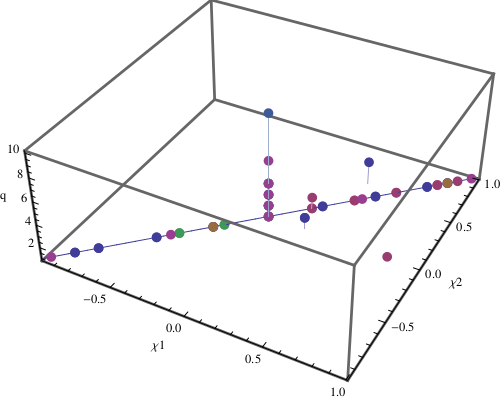
\includegraphics[width=0.95\linewidth]
{papers/mdc2013_submission/figure1.png}}
  \caption[Parameters of the NINJA-2 submissions]{
  \label{fig:ParameterSpace}
Mass ratio $q$ and dimensionless spins $\chi_i$ of the NINJA-2 hybrid
waveform submissions. Reproduced from \cite{Ajith:2012az}.
}
\end{figure}

Each waveform in the NINJA-2 waveform catalog consists of a PN 
portion modelling the early
inspiral, stitched to a numerical portion modelling the late inspiral,
merger and ringdown.  This ensures accurate modelling of the late
portions of the waveform while simultaneously ensuring that waveforms
are long enough to be scaled to masses as low as $10 M_\odot$ without
starting abruptly within the sensitive frequency band of the
detectors.  We require that for the NR portion of the waveform the
amplitude be accurate to within 5\% 
and the phase (as a function of gravitational-wave frequency)
have an accumulated uncertainty over the inspiral, merger and ringdown
of no more than 0.5 rad.  Since we do not have access to exact
waveforms we define ``accuracy'' by convergence of the numerical
waveforms as resolution and waveform-extraction radius are increased.
We also require at least five orbits of numerical data in order to
ensure robust blending with the PN portion.  No requirements were
placed on the hybridization itself, although it is known that
hybridization can introduce significant errors
\cite{MacDonald:2011ne, Santamaria:2010yb, Ohme:2011rm}.
It was
decided to limit NINJA-2 to systems without eccentricity, and with
black-hole spins parallel or anti-parallel
to the orbital angular momentum.  This
last condition avoids precession, which we do for two reasons; (i)
precession greatly complicates waveform phenomonology
and we prefer to first tackle a simpler subset which still maintains
the main features of binary evolution and merger; and (ii) at the
start of NINJA-2 the precessing-binary parameter space had been
sampled by only a handful of numerical simulations.  Waveforms were
submitted in the format described in~\cite{Brown:2007jx}, and data was
provided as strain decomposed into spherical harmonics of weight $-2$.
Groups were encouraged to submit modes beyond $(l,m)=(2,\pm 2)$
and many 
did so.  However the techniques to validate these higher modes
are a current research topic.  In order not to delay the NINJA-2
project it was decided to validate only the $(2,\pm 2)$ modes 
in~\cite{Ajith:2012az} and employ only these modes for the first
NINJA-2 analysis. Different groups employed different codes, as well
as different methods for solving initial conditions, dealing with
singularities, evolving Einstein's equations, and extracting
gravitational-wave information.  In addition different PN
approximants and different hybridization methods were used by
different groups in constructing the full hybrid waveforms. 
It was found that the
dominant source of disagreement between submissions was in the PN
portion, and in particular overlaps between submissions were greater
than 0.97 over the range of
masses, including regions sensitive to differences in hybridization
techniques. See~\cite{Ajith:2012az} for details.

The parameter space for aligned-spin BBH systems is four dimensional;
the masses and spin magnitudes of each of the two holes.  However, in
the absence of matter Einstein's equations possess a mass invariance,
and a solution obtained by numerical relativity or other method may be
trivially rescaled to any total mass.  We therefore eliminate total
mass from the parameter space of submissions leaving the ratio of the
two masses, denoted $q$, and the dimensionless spins denoted
$\chi_{1,2}$ which must lie between $-1 < \chi_{1,2} < 1$.

Tables~\ref{tab:ninja2_submissions1} and~\ref{tab:ninja2_submissions2} give a
summary of the submissions for systems where the masses of the two
black holes are equal and unequal, respectively. The first column of 
Tables~\ref{tab:ninja2_submissions1}
and~\ref{tab:ninja2_submissions2} gives a label for each waveform, to
ease referring to them in later sections.  These labels of the
form ``{\tt G2+20+20\_T4}'' are constructed as follows: The first letter
represents the group submitting the numerical simulation:
\begin{itemize}
\item[{\bf F}:] The numerical relativity group at Florida Atlantic University, 
also using the BAM 
code~\cite{Tichy:2010qa,Brugmann:2008zz,Marronetti:2007ya,Bruegmann:2003aw}.
\item[{\bf G}:] The Georgia Tech group using 
MayaKranc~\cite{Healy:2008js,Healy:2009ir,Bode:2009mt,Herrmann:2007ex,
Healy:2009zm,Bode:2011tq,Hinder:2007qu}
\item[{\bf J}:] The BAM (Jena) code, as used by the Cardiff-Jena-Palma-Vienna
  
collaboration~\cite{Husa:2007hp,Hannam:2007wf,Ajith:2009bn,Hannam:2010ec,
Brugmann:2008zz,Hannam:2007ik}
\item[{\bf L}:] The Lean Code, developed by Ulrich 
Sperhake~\cite{Sperhake:2006cy,Sperhake:2007gu}.
\item[{\bf Ll}:] The Llama code, used by the AEI group and the Palma-Caltech 
groups~\cite{Pollney:2010hs,Reisswig:2009rx,Pollney:2009yz}
\item[{\bf R}:] The group from Rochester Institute of Technology, using the
  LazEv code~\cite{Campanelli:2005dd,Lousto:2010tb,Lousto:2010qx,Nakano:2011pb}.
\item[{\bf S}:] The SXS collaboration using the SpEC 
code~\cite{Pfeiffer:2002wt,Scheel:2006gg,Lovelace:2011nu,Szilagyi:2009qz,
Lovelace:2010ne,Scheel:2008rj,SpECWebsite,Boyle:2007ft,Lindblom:2005qh,
Boyle:2009vi}.
\item[{\bf U}:] The group from The University of Illinois~\cite{Etienne:2008re}.
\end{itemize}
%
Immediately after this letter follows the mass-ratio $q=m_1/m_2$,
where the black holes are labeled such that $q\ge 1$.  Subsequently
are the components of the initial dimensionless spin along the orbital
angular momentum, multiplied by 100 (e.g. `+20' corresponds to $\hat
L\cdot \vec S_1 /m_1^2=0.2$) of the more massive and the less massive
black hole, respectively.
The label closes with the Taylor-approximant being used
for the PN portion of the waveform, with ``T1'' and ``T4'' representing
TaylorT1 and TaylorT4, respectively.  The Georgia Tech group submitted
four pairs of simulations where each pair simulates systems with identical 
physical parameters, stitched to the same PN approximant. These 
waveforms are not identical however as each simulation within a pair has a 
different number of NR cycles and was generated at a different resolution.  
These are distinguished by appending ``\_1'' and ``\_2'' to the label.

Each NR group verified that their waveforms met the minimum NINJA-2
requirements as described above.  The minimum-five-orbits requirement
was easily verified by inspection, and the amplitude and phase
uncertainties were estimated by convergence tests with respect to
numerical resolution and waveform-extraction radius.  The full catalog
was then verified by the NINJA-2 collaboration.  Submissions were inspected in
the time and frequency domains to identify any obvious problems caused
by hybridization or integration from the Newman-Penrose curvature
scalar $\psi_4$ to strain.  Where multiple simulations were available
for the same physical parameters these simulations were compared using
the matched-filter \emph{overlap}.  The inner product $\InnerProduct{s_1|s_2}$
between two real waveforms $s_1(t)$ and $s_2(t)$ is defined in 
Eq.~\ref{eq:overlap},
% %
% \begin{equation}
% \label{eq:InnerProduct}
%      \InnerProduct{s_1|s_2} 
%  = 4\, \Re \int_{0}^\infty df\,
%    \frac
%      {\tilde{s}_1(f) \tilde{s}_2^\star(f)}
%      {S_n(f)}
% \end{equation}
% %
% where $\tilde{x}$ denotes the Fourier transform of $x$
where $S_n(f)$ is the power spectral density, which was taken to
be the target sensitivity for the first advanced-detector runs,
referred to as the ``early aLIGO'' PSD. This is described in more detail in 
section \ref{sec:noise}.

The overlap is then
obtained by normalization and maximization over relative time and
phase shifts, $\Delta t$ and $\Delta \phi$. 
%
\begin{equation}
  \label{eq:OverlapDefinition}
  \Overlap{s_1, s_2} \define 
  \max_{\Delta t, \Delta \phi} \frac{\InnerProduct{s_1|s_2}}{
    \sqrt{\InnerProduct{s_1|s_1} \InnerProduct{s_2|s_2}}},
\end{equation}
%
which is the same as Eq.~\ref{eq:maxnormolap}.
The investigations in \cite{Ajith:2012az} demonstrated that
the submitted waveforms met the requirements as outlined above and in
addition were consistent with each other to the extent expected.  We
therefore conclude that these submissions model real gravitational
waves with sufficient accuracy to quantitatively determine how
data-analysis pipelines will respond to signals in next-generation
gravitational-wave observatories.

The NINJA-2 waveforms cover the 3-dimensional aligned-spin parameter
space rather unevenly, as indicated in figure~\ref{fig:ParameterSpace}.
The configurations available fall predominantly into two 1-dimensional
subspaces: (i) Binaries of varying mass-ratio, but with non-spinning
black holes.  (ii) Binaries of black holes with equal-mass and
equal-spin, and with varying spin-magnitude. Future studies, with additional 
waveforms covering the gaps that are clearly evident in 
figure~\ref{fig:ParameterSpace} 
and waveforms including 
precession~\cite{Campanelli:2008nk,Mroue:2013xna,Hinder:2013oqa}, 
would be useful to more fully understand the 
response of search codes across the parameter space, and would help to better 
tune analytical waveform models including inspiral, merger and ringdown phases.
%
\begin{table}
\caption[Submissions to NINJA-2]{
\label{tab:ninja2_submissions1}
Summary of the contributions to the NINJA-2 waveform catalog with $m_1
= m_2$.  Given are an identifying label, described in
section~\ref{sec:waveforms}, mass-ratio $q=m_1/m_2$ which is always
$1$ for these simulations, magnitude of the dimensionless spins
$\chi_i=S_i/m_i^2$, orbital eccentricity $e$, frequency range of
hybridization in $M\omega$, the number of numerical cycles from the
middle of the hybridization region through the peak amplitude, and the
post-Newtonian Taylor-approximant(s) used for hybridization.
}
%   \begin{indented}
%    \item[]
  \begin{tabular}{@{}rrrcrrcc}
      \hline
      Label & $q$ & $\chi_{1}$ & $\chi_{2}$ & $1000e$   & $100\,M\omega$ & \# NR 
& pN \\
      &    &     &            &            & hyb.range & cycles & Approx \\
      \hline
%       \mr
S1-95-95\_T1 & 1.0  &  -0.95  &  -0.95  &  1.00  &   3.3 -- 4.1  &  18.42  &  T1 
\\
J1-85-85\_T1 & 1.0  &  -0.85  &  -0.85  &  2.50  &   4.1 -- 4.7  &  12.09  & 
T1\\
J1-85-85\_T4 & & & & & & & T4 \\
J1-75-75\_T1 & 1.0  &  -0.75  &  -0.75  &  1.60  &   4.1 -- 4.7  &  13.42  & 
T1\\
J1-75-75\_T4 & & & & & & & T4 \\
J1-50-50\_T1 & 1.0  &  -0.50  &  -0.50  &  2.90  &   4.3 -- 4.7  &  15.12  & 
T1\\
J1-50-50\_T4 & & & & & & & T4 \\
S1-44-44\_T4 & 1.0  &  -0.44  &  -0.44  &  0.04  &   4.3 -- 5.3  &  13.47  &  T4 
\\
Ll1-40-40\_T1 & 1.0  &  -0.40  &  -0.40  &    &   6.1 -- 8.0  &  6.42  & T1\\
Ll1-40-40\_T4 & & & & & & & T4 \\
J1-25-25\_T1 & 1.0  &  -0.25  &  -0.25  &  2.50  &   4.5 -- 5.0  &  15.15  & 
T1\\
J1-25-25\_T4 & & & & & & & T4 \\
Ll1-20-20\_T1 & 1.0  &  -0.20  &  -0.20  &    &   5.7 -- 7.8  &  8.16  & T1\\
Ll1-20-20\_T4 & & & & & & & T4 \\
J1+00+00\_T1 & 1.0  &  0.00  &  0.00  &  1.80  &   4.6 -- 5.1  &  15.72  & T1\\
J1+00+00\_T4 & & & & & & & T4 \\
G1+00+00\_T4 &   &    &    &  3.00  &  5.5 -- 7.5  &  9.77  &  T4 \\
Ll1+00+00\_F2 &   &    &    &    &  5.7 -- 9.4  &  8.30  &  F2 \\
S1+00+00\_T4 &   &    &    &  0.05  &  3.6 -- 4.5  &  22.98  &  T4 \\
G1+20+20\_T4\_1 & 1.0  &  0.20  &  0.20  &  10.00  &   6.0 -- 7.5  &   6.77  &  
T4 \\ %MayaKranc_D10_a0.20_m77_nj.bbh.minimal
G1+20+20\_T4\_2 &      &        &        &   6.00  &   5.5 -- 7.5  &  10.96  &  
T4 \\ %MayaKranc_D12_a0.20_m103_nj.bbh.minimal
J1+25+25\_T1 & 1.0  &  0.25  &  0.25  &  6.10  &   4.6 -- 5.0  &  18.00  & T1\\
J1+25+25\_T4 & & & & & & & T4 \\
G1+40+40\_T4\_1 & 1.0  &  0.40  &  0.40  &  10.00  &   5.9 -- 7.5  &   7.70  &  
T4 \\ %MayaKranc_D10_a0.40_m90_nj.bbh.minimal
G1+40+40\_T4\_2 &      &        &        &   6.00  &   5.5 -- 7.5  &  12.02  &  
T4 \\ %MayaKranc_D12_a0.40_m103_nj.bbh.minimal
Ll1+40+40\_T1 &   &    &    &    &  7.8 -- 8.6  &  6.54  & T1\\
Ll1+40+40\_T4 & & & & & & & T4 \\
S1+44+44\_T4 & 1.0  &  0.44  &  0.44  &  0.02  &   4.1 -- 5.0  &  22.39  &  T4 
\\
J1+50+50\_T1 & 1.0  &  0.50  &  0.50  &  6.10  &   5.2 -- 5.9  &  15.71  & T1\\
J1+50+50\_T4 & & & & & & & T4 \\
G1+60+60\_T4\_1 & 1.0  &  0.60  &  0.60  &  12.00  &   6.0 -- 7.5  & 8.56  &  T4 
\\   %MayaKranc_D10_a0.60_m77_nj.bbh.minimal
G1+60+60\_T4\_2 &      &        &        &   5.00  &   5.5 -- 7.5  &  13.21  &  
T4 \\ %MayaKranc_D12_a0.60_m103_nj.bbh.minimal
J1+75+75\_T1 & 1.0  &  0.75  &  0.75  &  6.00  &   6.0 -- 7.0  &  14.03  & T1\\
J1+75+75\_T4 & & & & & & & T4 \\
G1+80+00\_T4 & 1.0  &  0.80  &  0.00  &  13.00  &   5.5 -- 7.5  &  12.26  &  T4 
\\ %MayaKranc_D10_a0.80_m90_nj.bbh.minimal
G1+80+80\_T4\_1 & 1.0  &  0.80  &  0.80  & 14.00  &   5.9 -- 7.5  &  9.57  &  T4 
\\ %MayaKranc_D12_a0.80_m103_nj.bbh.minimal
G1+80+80\_T4\_2 &      &        &        &  6.70  &   5.5 -- 7.5  & 14.25  &  T4 
\\
J1+85+85\_T1 & 1.0  &  0.85  &  0.85  &  5.00  &   5.9 -- 6.9  &  15.36  & T1\\
J1+85+85\_T4 & & & & & & & T4 \\
U1+85+85\_T1 &   &    &    &  20.00  &  5.9 -- 7.0  &  15.02  &  T1 \\
G1+90+90\_T4 & 1.0  &  0.90  &  0.90  &  3.00  &   5.8 -- 7.5  &  15.05  &  T4 
\\
S1+97+97\_T4 & 1.0  &  0.97  &  0.97  &  0.60  &   3.2 -- 4.3  &  38.40  &  T4 
\\
      \hline
%       \ms\bhline\ms
    \end{tabular}
%   \end{indented}
\end{table}



%
\begin{table}
\caption[Submissions to NINJA-2]{
\label{tab:ninja2_submissions2}
Summary of the contributions to the NINJA-2 waveform catalog with $m_1
> m_2$.  Given are an identifying label, described in 
section~\ref{sec:waveforms}, 
mass-ratio $q=m_1/m_2$
magnitude of the dimensionless spins $\chi_i=S_i/m_i^2$, orbital
eccentricity $e$, frequency range of hybridization in $M\omega$, the
number of numerical cycles from the middle of the hybridization region
through the peak amplitude, and the post-Newtonian Taylor-approximant(s)
used for hybridization.
}
%   \begin{indented}
%     \item[]
  \begin{tabular}{@{}rrrcrrcc}
%       \ms\bhline\ms
      \hline
      Label & $q$ & $\chi_{1}$ & $\chi_{2}$ & $1000e$   & $100\,M\omega$ & \# NR 
& pN \\
      &    &     &            &            & hyb.range & cycles & Approx \\
      \hline
%       \mr
J2+00+00\_T1 & 2.0  &  0.00  &  0.00  &  2.30  &   6.3 -- 7.8  &  8.31  & T1\\
J2+00+00\_T4 & & & & & & & T4 \\
G2+00+00\_T4 &   &    &    &  2.50  &  5.5 -- 7.5  &  10.42  &  T4 \\
Ll2+00+00\_F2 &   &    &    &    &  6.3 -- 9.4  &  7.47  &  F2 \\
S2+00+00\_T2 &   &    &    &  0.03  &  3.8 -- 4.7  &  22.34  &  T2 \\
G2+20+20\_T4 & 2.0  &  0.20  &  0.20  &  10.00  &   5.6 -- 7.5  &  11.50  &  T4 
\\
J2+25+00\_T1 & 2.0  &  0.25  &  0.00  &  2.00  &   5.0 -- 5.6  &  15.93  & T1\\
J2+25+00\_T4 & & & & & & & T4 \\
J3+00+00\_T1 & 3.0  &  0.00  &  0.00  &  1.60  &   6.0 -- 7.1  &  10.61  & T1\\
J3+00+00\_T4 & & & & & & & T4 \\
S3+00+00\_T2 &   &    &    &  0.02  &  4.1 -- 5.2  &  21.80  &  T2 \\
F3+60+40\_T4 & 3.0  &  0.60  &  0.40  &  1.00  &   5.0 -- 5.6  &  18.89  &  T4 
\\
J4+00+00\_T1 & 4.0  &  0.00  &  0.00  &  2.60  &   5.9 -- 6.8  &  12.38  & T1\\
J4+00+00\_T4 & & & & & & & T4 \\
L4+00+00\_T1 &   &    &    &  5.00  &  5.1 -- 5.5  &  17.33  &  T1 \\
S4+00+00\_T2 &   &    &    &  0.03  &  4.4 -- 5.5  &  21.67  &  T2 \\
S6+00+00\_T1 & 6.0  &  0.00  &  0.00  &  0.04  &   4.1 -- 4.6  &  33.77  &  T1 
\\
R10+00+00\_T4 & 10.0  &  0.00  &  0.00  &  0.40  &   7.3 -- 7.4  &  14.44  &  T4 
\\
      \hline
%       \ms\bhline\ms
    \end{tabular}
%   \end{indented}
\end{table}

\section{Modified Detector Noise}
\label{sec:noise}

We stress here that the production of the final noise data set, which emulated data
that will be taken by second generation gravitational wave observatories, 
was performed by members of the NINJA-2 collaboration who are not the author 
of this dissertation.  
However, we find it useful to present a brief desrciption of the same here.
The noise emulation 
was accomplished by recoloring data taken from the initial LIGO and Virgo 
instruments to predicted 2015 -- 2016 sensitivities. Recoloring initial LIGO 
and 
Virgo data allows the non-Gaussianity and non-stationarity of that data to be 
maintained.

\begin{figure}
\centering
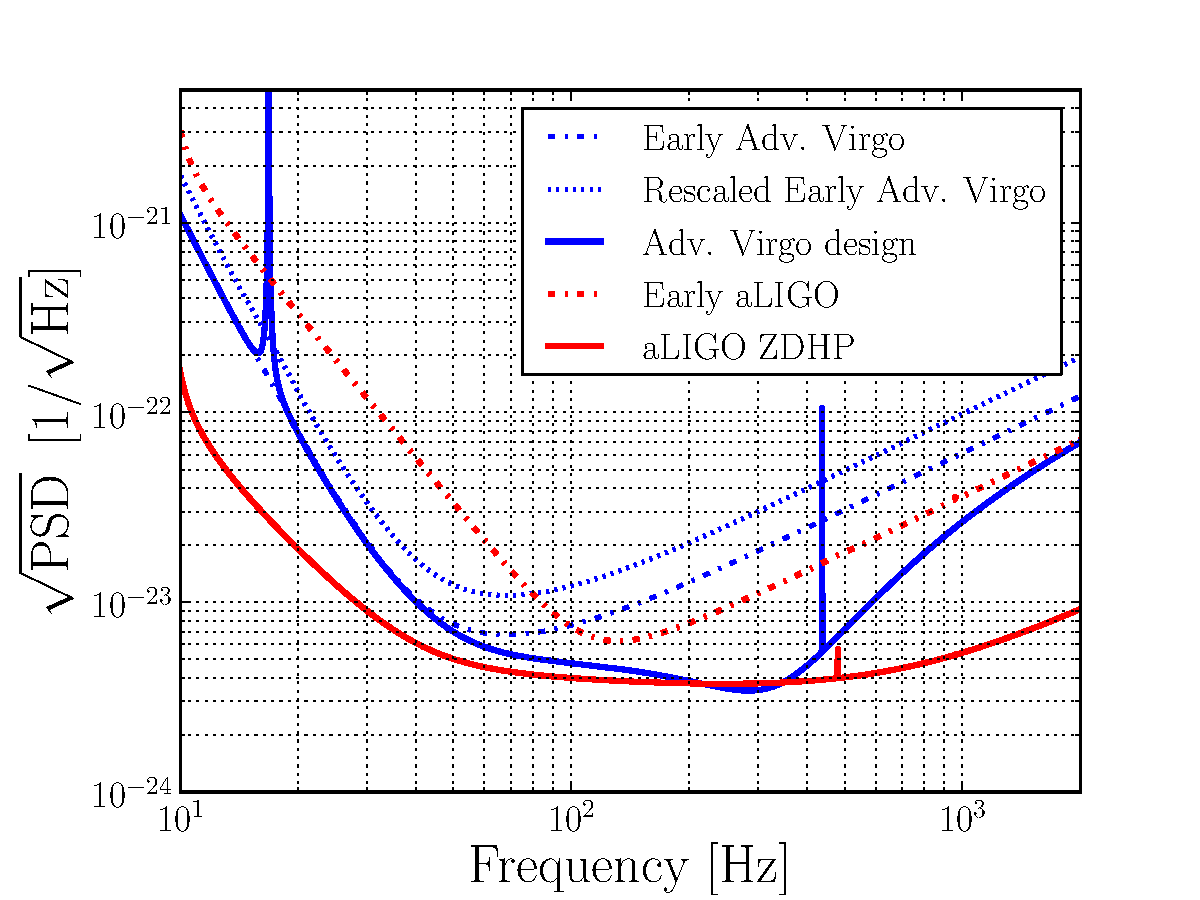
\includegraphics[width=0.85\textwidth]
{papers/mdc2013_submission/figure2A}
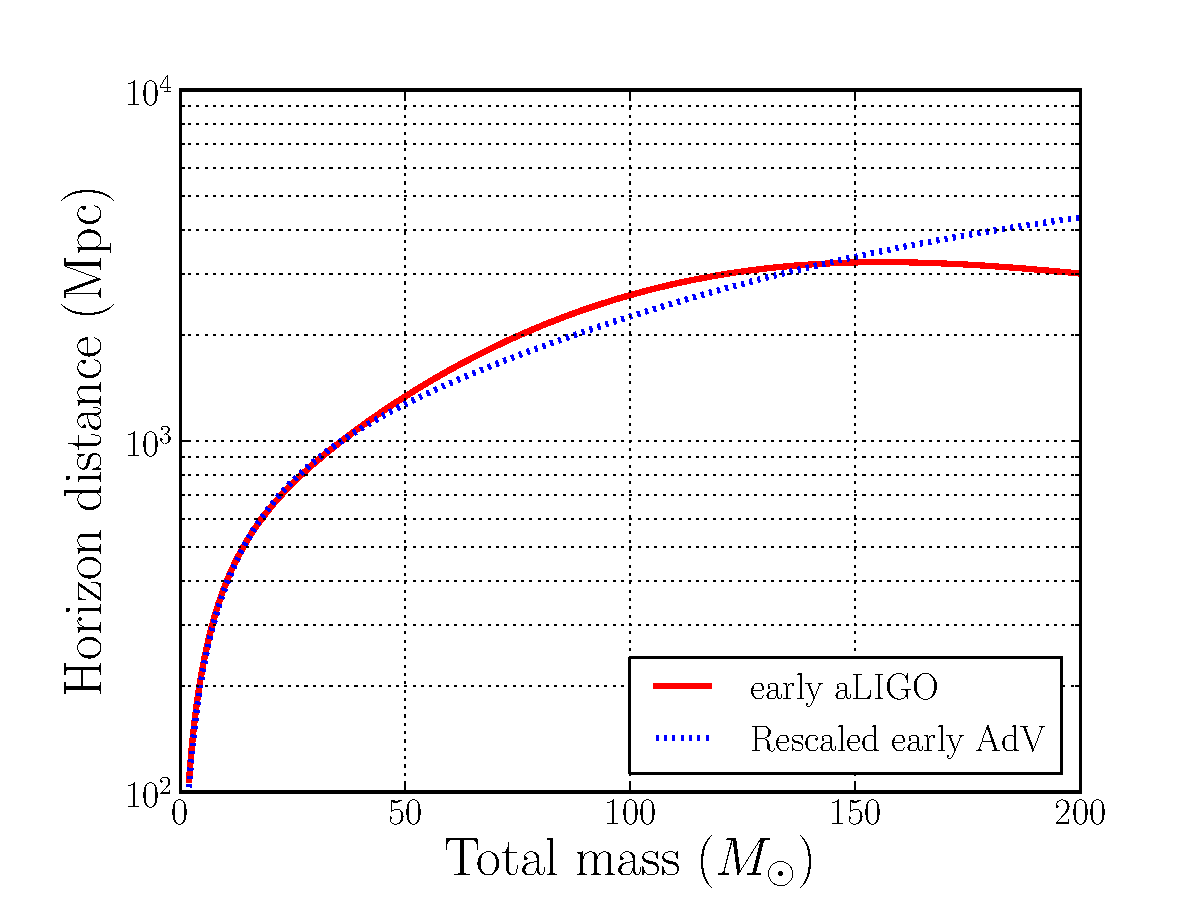
\includegraphics[width=0.85\textwidth]
{papers/mdc2013_submission/figure2B}
\caption{\label{fig:NOISE_design_spectra}
Top: predicted sensitivity curves for aLIGO and
AdV. Shown are both the design curves and predicted 2015 -- 2016
\emph{early} sensitivity curves. Also shown is the early AdV noise curve 
rescaled such that the horizon distance for a (10 $M_{\odot}$, 10 $M_{\odot}$) 
binary system is equal to that obtained with the early aLIGO noise 
curve. Bottom: Horizon distance as a function of observed total mass for the 
early aLIGO and rescaled early AdV sensitivity curves. This plot is 
made considering only equal mass, non-spinning systems and calculated using the 
\eob ~\cite{Pan:2011gk} waveform approximant. Results in this paper are 
generated from the early aLIGO noise curve and the rescaled early AdV curve.}
\end{figure}

The predicted sensitivity curves of the advanced detectors as a function of
time can be found in the living document
\cite{Aasi:2013wya}. For this work we are interested in the
sensitivity of the advanced detectors in 2015 -- 2016 and used a previous 
prediction of the sensitivity curves for this time period as given in
\cite{LV_early_noisecurves} and shown in the left panel of figure 
\ref{fig:NOISE_design_spectra}.
These curves were used as the updated predictions given in 
\cite{Aasi:2013wya} were not available when we began this study.
We refer to the 2015 -- 2016 predicted noise curves as the \emph{early} 
sensitivity curves.
It is clear from the figure that the predicted
sensitivity of early AdV is significantly greater than 
that of the early aLIGO curve, when using the predictions given in 
\cite{LV_early_noisecurves}. In the right panel of figure 
\ref{fig:NOISE_design_spectra} we
show the distance at which optimally oriented, optimally located,
non-spinning, equal mass binaries would be detected with a
signal-to-noise ratio (SNR) of 8 using both noise curves.
This is commonly referred to as the \emph{horizon distance}. The early AdV 
noise curve was rescaled
by a factor of 1.61 so that the sensitive distance for a
(10 $M_{\odot}$, 10 $M_{\odot}$) binary merger would be equal to the early aLIGO
noise curve. This rescaling was found to better reflect the updated predicted
sensitivities presented in \cite{Aasi:2013wya}. The results in this 
chapter were generated using the early aLIGO and rescaled early AdV sensitivity 
curves.

As with the initial science runs, we expect data taken from
these detectors, in the absence of gravitational-wave signals, to be neither
Gaussian nor stationary. It is important that search pipelines demonstrate
an ability to deal with these features. To simulate data with 
advanced detector sensitivities and with
realistic non-Gaussian and non-stationary features, we chose to use
data recorded by initial LIGO and Virgo and recolor that data to the
predicted early sensitivity curves of aLIGO and AdV. The data we
chose to recolor was data taken during LIGO's sixth science run and Virgo's
second science run.

% The procedure for producing such \emph{recolored data} was accomplished in the
% following steps, which were conducted separately for the two LIGO detectors and
% Virgo.
% 
% \begin{itemize}
%  \item Identify a two-month duration of initial detector data to be 
% recolored
%  \item Measure the power spectral density (PSD) for each distinct section 
% of science mode data using the PSD estimation routines in the \texttt{lal} 
% software package \cite{LAL}.
%  \item Calculate an \emph{average PSD} over the two month period by taking, for
% every discrete value of frequency recorded in the PSDs, the median value over
% each of the PSDs in the set.
%  \item Remove any sharp ({\it line}-like) features from the resulting PSD and from the predicted
% early noise curves. This is done because it is difficult to remove or introduce 
% line features from the data without introducing unwanted artifacts. Therefore 
% it is simpler to remove line features in the PSDs, which will have the effect 
% of preserving the line features of the original data into the recolored 
% data.
%  \item For each frequency bin, record the median value of the PSD over each 
% section of science mode
%  \item Take the ratio of the median PSD and the predicted early advanced
% detector noise curve.
%  This is the reweighting to be used when recoloring.
%  \item Using the time domain filtering abilities of the \texttt{gstlal}
% software package \cite{GSTLAL}, recolor the data using this reweighting factor.
% \end{itemize}

\begin{figure}
\centering
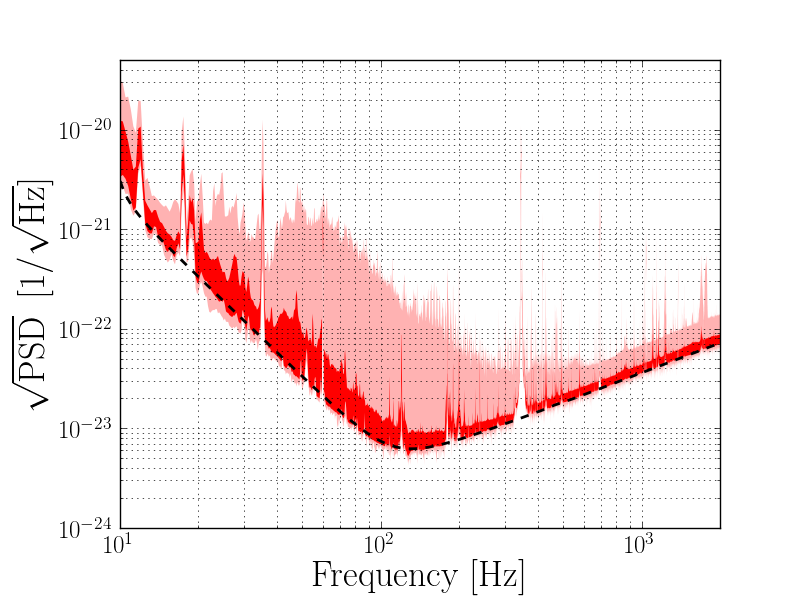
\includegraphics[width=0.495\textwidth]
{papers/mdc2013_submission/figure3A.png}
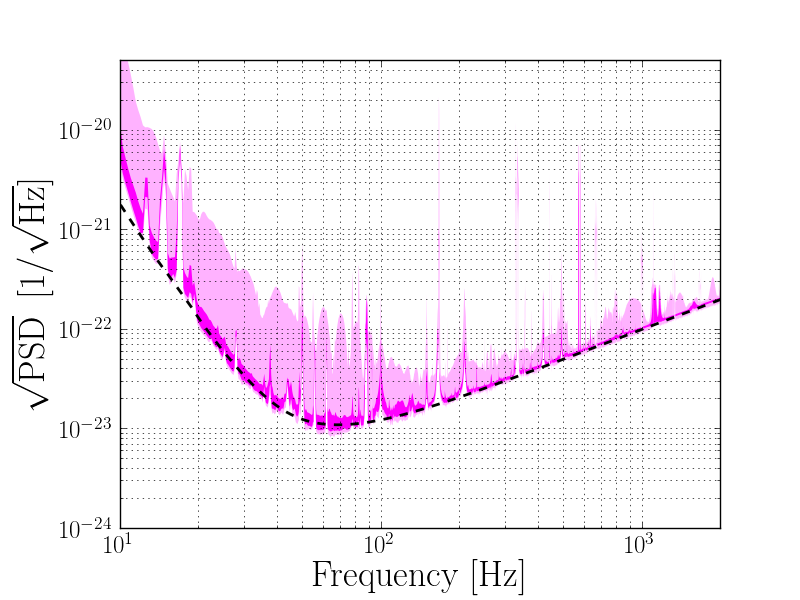
\includegraphics[width=0.495\textwidth]
{papers/mdc2013_submission/figure3B.png}
\caption{\label{fig:NOISE_recolored_sens}
Sensitivity curves of the recolored data for the LIGO Hanford detector (left)
and the Virgo detector (right). In both cases the black dashed line shows the
predicted 2015 -- 2016 sensitivity curve (with the scaling factor added for
Virgo). The dark colored region indicates the range between the 10 \% and 90 \%
quantiles of the PSD over time. The lighter region shows the range
between the minimum and maximum of the PSD over time.}
\end{figure}

In figure \ref{fig:NOISE_recolored_sens} we show some examples of the PSDs
obtained from recoloring the data and compare with
the predicted sensitivity curves. As there are some small stretches of data in
the original science runs where the sensitivity was significantly different
from the average, we show the 10 \% and 90 \% quantiles as well as the maximum 
and
minimum values for the PSD of the recolored data. We notice that the sensitivity
of the detector still varies with time, as in the initial data, and that the
lines in the initial spectra are still present.

\begin{figure}
\centering
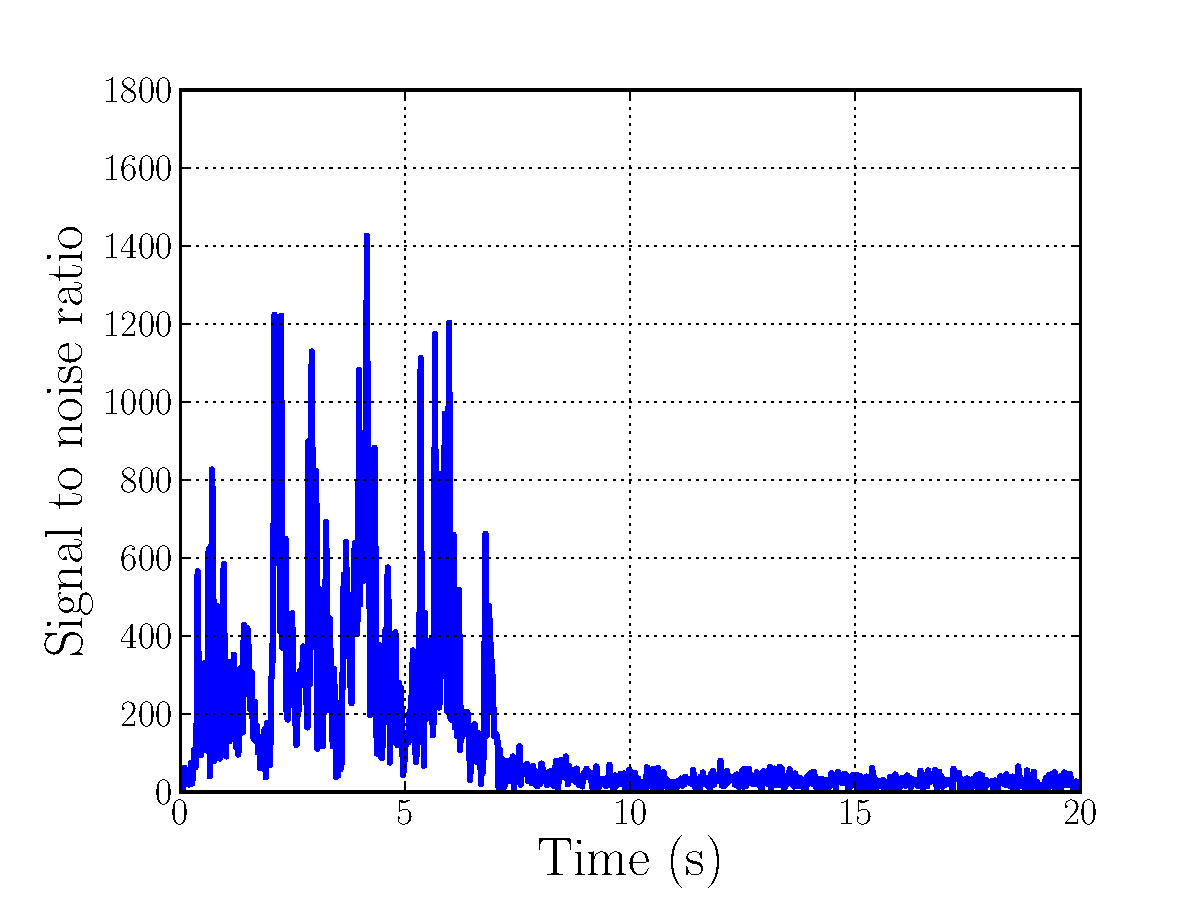
\includegraphics[width=0.495\textwidth]
{papers/mdc2013_submission/figure4A}
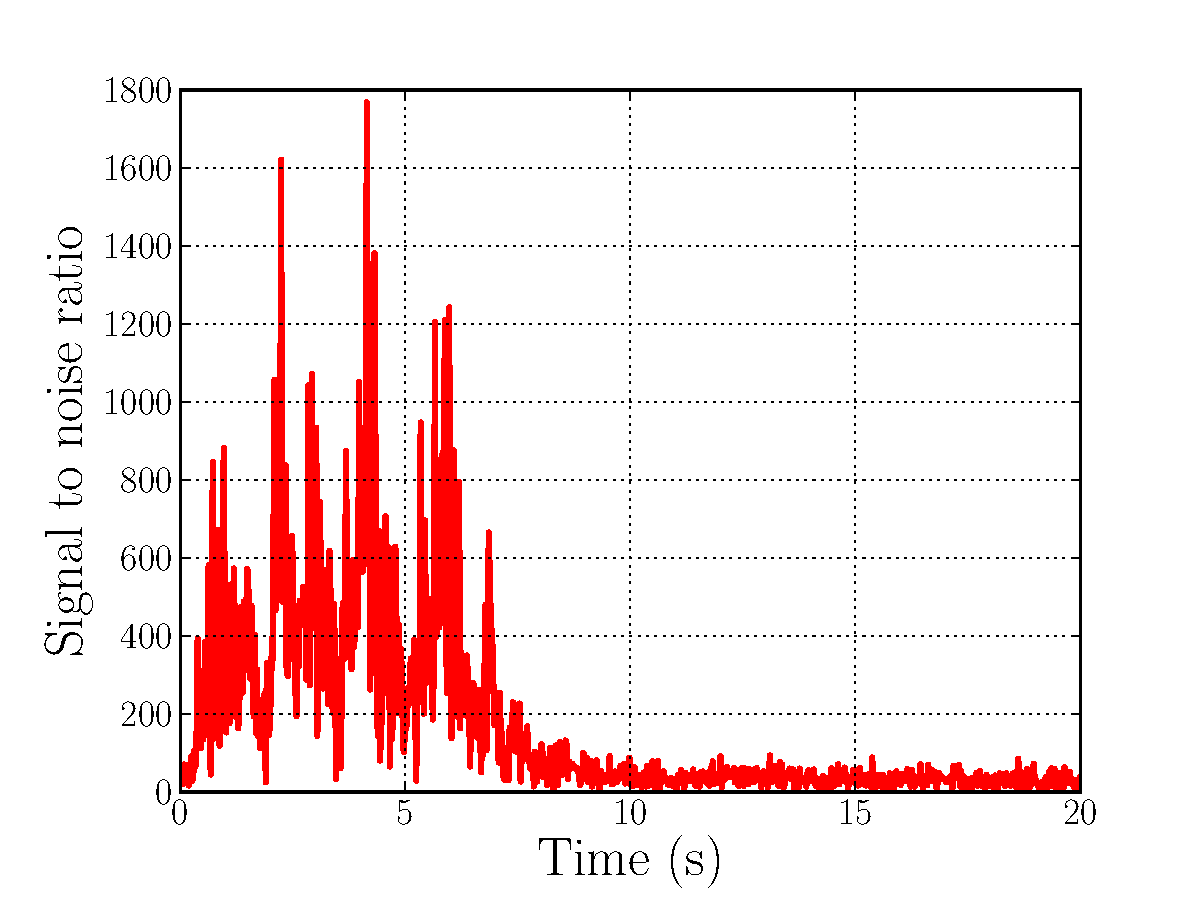
\includegraphics[width=0.495\textwidth]
{papers/mdc2013_submission/figure4B}
\caption{\label{fig:NOISE_recolored_glitch}
SNR time series in a 20 s window around a known glitch in the original data
(left) and in the recolored data (right). While the SNR time series clearly
change, the primary features of the glitch are preserved across the recoloring
procedure. These SNR time series were obtained by matched-filtering a short 
stretch of recolored and original data against a (23.7,1.3) $M_{\odot}$ 
template.}
\end{figure}

Non-Gaussian features present in the original data will still be present in
the recolored data, albeit distorted by the recoloring process.
An example of this is shown in figure
\ref{fig:NOISE_recolored_glitch} where we show the SNR time-series around a
known glitch in both the original and recolored data. While the recoloring does
have some effect on the glitch, the two SNR time series are very comparable. As
in searches on the original data, we attempt to mitigate the effect of such
features. A set of \emph{data quality flags} were created for the initial 
detector
data \cite{Aasi:2012wd,LIGOS6Detchar}.
These attempt to flag times where a known instrumental or
environmental factor, which is known to produce non-Gaussian artifacts in the
resulting strain data, was present. To simulate these data quality flags in our
recolored data we simply used the same flags that were present in the original
data and apply them to the recolored data.

\section{Injection Parameters}
\label{sec:parameters}

As an unbiased test of the process through which candidate 
events are identified for BBH waveforms, 7 BBH waveforms were added to the 
recolored data. This was performed by one member of the collaboration, who is 
not the author of this dissertation.
We were aware that ``blind injections'' had been
added, however the number and parameters of these simulated signals were not 
disclosed until the analysis was completed. This was similar to blind 
injection tests conducted by the LIGO and Virgo collaborations in their latest 
science runs \cite{Colaboration:2011np}.
These injections are self-blinded to ensure that no bias from knowing the
parameters of the signal, or indeed whether a candidate event is a signal or a 
noise artifact, affects the analysis process.

The 7 waveforms added to the data were taken from the numerical
relativity simulations discussed in section \ref{sec:waveforms}. The parameters
of the blind injections are given in Table \ref{tab:blindsigs}. The distribution
of physical parameters used in these blind injections was not intended to
represent any physical distribution. Instead, the injections were chosen to 
test 
the ability
to recover BBH systems across a wide range of parameter space. 
% We describe the results of searches for these blind injections in section 
% \ref{sec:searches} and of parameter estimation studies on these signals in 
% section \ref{sec:param_estimation}.

\begin{table}
\caption{\label{tab:blindsigs} The details of the blind injections that were
added to the NINJA-2 datasets prior to analysis. In this table the Event ID
will be used throughout the paper to refer to specific injections. The network
SNR of each injection is denoted by $\rho_{\mathrm N}$. This is the sum of the
overlaps of the injection with itself in each detector, using $30\,$Hz as the
starting frequency in the overlap integrals. $M$ denotes the total mass and $q$
the mass ratio.  $\chi$ denotes the spin on \emph{each} black hole, in all 7
cases both black holes in the binary had the same spin. RA and dec give the
right ascension and declination of the signals respectively.  Dist. denotes the
distance to the source. Detectors online lists the detectors for which data is
present at the time of signal. Hybridization range gives the range of
frequencies in which the signal is hybridized between the post-Newtonian and
numerical components.  Waveform label indicates which numerical waveform was
used, as shown in Tables \ref{tab:ninja2_submissions1} and
\ref{tab:ninja2_submissions2}.  }
\resizebox{\textwidth}{!}{%
\begin{tabular}{@{}ccccccccccc}
% \ms\bhline\ms
Event & Waveform   &                    &      &  
  $M$                   &          &  RA     &  Dec.   &  Dist.  &  Detectors & 
Hybrid   \\
ID    & label      & $\rho_{\mathrm N}$ & $q$  &
  ($\mathrm{M}_\odot$)  &  $\chi$  &  (rad)  &  (rad)  &  (Mpc)  &  Online    & 
Range (Hz)        \\
% \mr
1 & J4+00+00\_T4  & 23.9 & 4  &  124   &  0.00  &  1.26  &  -0.76  &  569  &  
HLV 
 & 15 -- 18 \\
2 & Ll1-20-20\_T4 & 14.1 & 1  &  35.5  & -0.20  &  1.70  &  -0.03  &  244  &  
HLV 
 & 52 -- 71 \\
3 & Ll1+40+40\_T4 & 16.2 & 1  &  14.4  &  0.40  &  4.18  &  0.07  &  170  &  HLV 
 
& 175 -- 193 \\
4 & G2+20+20\_T4 & 15.1 & 2  &  26.8  &  0.20  &  2.19  &  -0.36  &  247  &  LV  
 
& 68 -- 90 \\
5 & L4+00+00\_T1 & 19.2 & 4  &  19.1  &  0.00  &  1.68  &  0.14 &  83   &  HV  & 
 
86 -- 93 \\
6 & J1+25+25\_T4 & 16.9 & 1  &  75.7  &  0.25  &  4.68  &  0.49 &  854  &  HV  
& 
20 -- 21 \\
7 & J1-75-75\_T1 & 9.8 & 1  &  19.3  & -0.75  &  0.81  &  -0.07 &  292  &  HLV  
& 69 -- 79 \\
% \ms\bhline\ms
\end{tabular}}
\end{table}

% As well as these blind injections, a large number of (non-blind) simulated 
% signals were subsequently analyzed to obtain sufficient statistics to adequately
% evaluate the sensitive distances at which the NR waveforms could be detected 
% in the early aLIGO and early AdV simulated data sets. As mentioned in 
% section~\ref{sec:waveforms}, 
% each of the NR waveforms is valid only at the values of mass ratio and 
% dimensionless spins for which it was generated. However, it is possible to 
% change the total mass, which just rescales the waveform, and the various 
% orientation and location parameters, which will only affect the overall phase 
% and amplitude of the signal. For each of the 60 NR 
% waveforms given in Table~\ref{tab:ninja2_submissions1} and used in results in 
% section \ref{sec:sensitivity}, a set of $\sim42000$ 
% simulated signals was generated, necessarily with mass ratios and        
% spins that have values corresponding to the given NR waveform. The total mass 
% was chosen from a uniform 
% distribution between 10 and 100 $M_{\odot}$. The simulations were 
% distributed uniformly in distance, however they were not injected beyond a 
% distance where they could not possibly be detected. The mass-dependent maximum 
% distance that we chose to use is given by
% %
% \begin{equation}
%  D_{\mathrm{max}} = \left(\frac{\mathcal{M}}{1.219 M_{\odot}}\right)^{5/6}
%  \unit[175]{Mpc}.
% \end{equation}
% %
% Here $1.219 M_{\odot}$ is the chirp mass of a $(1.4+1.4)M_{\odot}$ binary 
% system. The factor of $\mathcal{M}^{5/6}$ describes, to leading order, how 
% the SNR of the inspiral-only portion of a compact-binary 
% merger at fixed distance will scale with mass when the inspiral is 
% bandwidth-limited~\cite{Peters:1963ux,Allen:2005fk}. $175$ Mpc is chosen 
% because 
% it is larger than the distance at which it would be possibly to detect 
% a $(1.4+1.4)M_{\odot}$ binary merger with the early noise curves. However, to 
% include a large margin for safety $\sim7000$ of the signals were generated with 
% chirp-weighted distances between $175$ and $350$ Mpc. The orbital 
% orientations, polarization angles and sky directions are all chosen from 
% isotropic distributions. The signal coalescence times are drawn from a uniform 
% distribution within our analysis window. Coalescence times were limited to 
% times where at least two observatories were operating and no data-quality flags 
% were active. The results of analyses on the non-blind simulated signals are 
% given in section~\ref{sec:sensitivity}.

\section{Search Pipelines}
\label{sec:pipelines}

The goal of this work was to evaluate the detection sensitivity to
binary black hole systems, modelled from the latest numerical
simulations, using the search pipelines that were used to search for
gravitational-wave transient signals in data taken during the final
initial LIGO and Virgo joint observing run.  The two pipelines that
were used to do this were the dedicated compact binary coalescence
(CBC) search pipeline ``\ihope{}'' \cite{Abbott:2009tt, Abbott:2009qj,
Abadie:2011kd, Colaboration:2011np, Aasi:2012rja, Babak:2012zx}
and the unmodelled burst pipeline ``Coherent WaveBurst'' (cWB)
\cite{Abbott:2007wu, Abadie:2010mt, Abadie:2012rq, Virgo:2012aa}. 
In this dissertation, we will focus on the modeled \ihope{} pipeline.
The \ihope{} pipeline was developed as a search pipeline for detecting
compact binary mergers. It employs a matched-filtering algorithm
against a bank of template waveforms~\cite{Babak:2012zx}. 
It was used to search for CBC systems (not just binary black
holes) with component masses $\in [1,99]\, \mathrm{M}_{\odot}$. 
% As a
% complement to template-based specialized searches, cWB was developed
% as an all-purpose un-modeled search pipeline, hence, it does not
% require \emph{a priori} knowledge of the signal waveforms. It is
% better suited for burst signals spanning a small time-frequency
% volume. Moreover, due to the lack of model constraints, cWB is more
% adversely affected by background noise than matched-filter searches.
% Past simulation studies with initial LIGO sensitivity curves have
% shown that cWB was sensitive to CBC mergers with total masses $\in
% [25,500]\, \mathrm{M}_{\odot}$ over wide regions of the binary
% parameter space \cite{Pankow:2009nx}.

In addition to the \ihope{} and cWB detection pipelines parameter 
estimation algorithms were used to provide estimates of the parameters of
compact binary systems observed with the detection algorithms. 
However, we will not focus on those here.
In this section we provide a brief overview of the detection 
pipeline \ihope{}.
The results of running the \ihope{} searches on the data containing the NINJA-2
blind injections are presented in section \ref{sec:searches}.

% \subsection{Coherent WaveBurst}
% \label{ssec:cwb_pipelines}
% 
% Coherent WaveBurst is a multi-resolution algorithm for coherent
% detection and reconstruction of gravitational wave
% bursts~\cite{Klimenko:2008fu}. The cWB algorithm has been used in
% various LIGO-Virgo burst searches
% \cite{Abbott:2007wu,Abadie:2010mt,Abadie:2012rq} and more recently in
% the search for intermediate mass black hole binaries
% \cite{Virgo:2012aa}.  Within the framework of the constrained maximum
% likelihood analysis \cite{Klimenko:2008fu}, cWB identifies GW signals
% in data from multiple detectors and provides estimates of the signal
% parameters, e.g. sky location and waveforms.  Along with the
% reconstruction of un-modeled burst signals, which imply random
% polarization, cWB can perform loosely modeled likelihood analyses
% assuming different polarization states, i.e.\ elliptical, linear or
% circular.
% 
% The NINJA2 cWB analysis uses the elliptical polarization constraint 
% \cite{Pankow:2009nx,Virgo:2012aa} and searches for signals in the frequency 
% band from 32 Hz to 1024 Hz. The analysis is performed in several steps: first, 
% the data streams from all GW detectors are processed with the Meyer's wavelet 
% transformations with 6 different  time-frequency resolutions of 
% $ 4\times1/8$, $8\times1/16$, $16\times1/32$, $32\times1/64$, 
% $64\times1/128$, $128\times1/256$ [Hz $\times$ s]. Then the data are 
% conditioned 
% with a linear predictor error filter to remove power lines, violin modes 
% and other predictable data components. Triggers are reconstructed as the 
% coherent
% sets of samples (pixels) identified in the time-frequency data. For each 
% trigger the coherent 
% statistics are then computed. These include the network correlation 
% coefficient, ${cc}$ and the network energy disbalance, ${\Lambda}$, which are 
% used to enable the signal consistency selection cuts. The cWB detection 
% statistic is the coherent network amplitude, $\eta$, which is used to rank the 
% events and thereby establish the significance against a sample of 
% background events obtained with the time-shift analysis 
% \cite{Klimenko:2008fu,Virgo:2012aa,Pankow:2009nx}. 
% This shifting procedure is typically performed 
% thousands of times in order to accumulate sufficient statistics.

\subsection{\ihope{}}
\label{ssec:ihope_pipelines}

The \ihope{} pipeline is designed to search for gravitational waves
emitted by coalescing compact binaries~\cite{Babak:2012zx}. It has been
optimized for and used in LIGO and Virgo GW searches over the past 
decade~\cite{Abbott:2007xi, Abbott:2009tt, Abbott:2009qj, Abadie:2010yb, 
Colaboration:2011np, Aasi:2012rja}, and also in the mock Laser 
Interferometer Space Antenna (LISA) data 
challenges~\cite{Babak:2008aa}. The NINJA-2 \ihope{} analysis uses the same 
pipeline-tuning that was used in the searches performed during 
the final initial LIGO and Virgo joint observing 
run~\cite{Colaboration:2011np}.

The pipeline matched-filters the detector data against a bank of
analytically modelled compact binary merger 
waveforms~\cite{Allen:2005fk,Babak:2012zx}. Only nonspinning compact binary 
merger signals are used as filters and the bank is created so as to densely 
sample the range of possible binary masses~\cite{Babak:2006ty}.
For each detector, the filtering stage produces 
a sequence of \textit{triggers} which are plausible events with a high 
signal to noise ratio SNR $\rho$. The algorithm proposed 
in~\cite{Robinson:2008un} is used to keep only those that are found coincident
in more than one detector across the network, which helps remove triggers due to 
noise. 
Knowledge of the instrument and its environment is used to further exclude
triggers that are likely due to non-Gaussian noise transients, or 
\textit{glitches}. Periods of heightened glitch rate are
removed (\emph{vetoed}) from the analysis. The time periods where the rate of 
glitches is elevated are divided into $3$ \emph{veto categories}. Periods of 
time flagged by category 1 and 2 vetoes are
not included in the analysis as known couplings exist between instrumental
problems and the gravitational-wave channel during these periods. Periods of
time vetoed at category 3 are \emph{likely} to have instrumental problems. A
strong gravitational-wave signal can still be detected during category 3 times,
but including these periods in the background estimate can compromise our
ability to detect weaker signals in less glitchy periods of time. For this
reason the search is performed both before and after category 3 vetoes are 
applied. The significance of events
that survived category 1-3 vetoes were calculated using the background that also
survived categories 1-3. The significance of events that survived category 2
but were vetoed at category 3 were calculated using background that survived
categories 1-2.

Signal based 
consistency measures further help distinguish real signals from background noise
triggers in those that are not vetoed and pass the coincidence test. 
The $\chi^{2}$ statistic proposed in~\cite{Allen:2004gu} quantifies the 
disagreement in the frequency evolution of 
the trigger and the waveform template that accumulated the highest SNR
for it, cf.\ Eq.~(4.14) of~\cite{Allen:2004gu}. We weight the SNR with this
statistic to obtain the \textit{reweighted} SNRs $\hat{\rho}$ 
for all coincident triggers. 
The exact weighting depends on the mass range the search is focused on, cf.\
Eq.~(17,18) of~\cite{Babak:2012zx}. The reweighted SNR is used as the
ranking statistic to evaluate the significance, and thus the false alarm rate 
(FAR), of all triggers. 

% Following the division of the mass-parameter space used 
% in~\cite{Colaboration:2011np, Aasi:2012rja}, we performed both \emph{low 
% mass} and \emph{high mass} \ihope{} searches on the NINJA-2 data. 
The low-mass search focused on binaries with $2M_\odot
\leq m_{1}+m_{2} < 25M_\odot$, and used frequency domain $3.5$PN 
waveforms as templates~\cite{Blanchet:2001ax, Blanchet:2001aw, Blanchet:2004ek}.
% The high-mass search instead focused on the mass-range 
% $25M_\odot \leq m_{1}+m_{2} < 100M_\odot$, and used the effective-one-body
% inspiral-merger-ringdown model calibrated to numerical relativity, as described 
% in~\cite{Buonanno:2007pf}. The exact $\chi^2$-weighting used to define the
% re-weighted SNR varied between the two analyses~\cite{Babak:2012zx}. 
The significance of the triggers found was estimated as follows.
All coincident triggers are divided into $4$ 
categories, i.e.\ HL, LV, HV and HLV, based on the detector combination they are 
found to be coincident in~\cite{Colaboration:2011np}. They are further divided 
into
$3$ \textit{mass}-categories based on their chirp mass
$\mathcal{M}_{c}=(m_{1}m_{2})^{3/5}(m_{1}+m_{2})^{-1/5}$ for the low-mass 
search, and $2$ categories based on their template duration for the high-mass 
search~\cite{Colaboration:2011np}. The rate of background noise triggers, or 
\textit{false alarms}, has been found to be significantly higher for shorter 
signals from more massive binaries, and also to be different depending on the 
detector combination, and these categorizations help segregate these effects 
for estimation of the background~\cite{Colaboration:2011np,Babak:2012zx}. 

For all the triggers the combined
re-weighted SNR $\hat{\rho}$ is computed, which is the quadrature sum of 
re-weighted SNRs across the network of detectors. All triggers are then 
ranked according to their $\hat{\rho}$ in each of the mass/duration and 
coincidence sub-categories independently, allowing us to estimate the 
trigger false alarm rate (FAR) at a given threshold $\hat{\rho}=\hat{\rho}_{0}$.
This is described by 
\begin{equation}\label{eq:FARdef}
\mathrm{FAR}~(\hat{\rho}_{0}) \simeq \frac{N(\hat{\rho}\geq 
\hat{\rho}_{0})}{T_{c}},
\end{equation}
i.e.\ the number of background noise triggers in a given coincidence 
sub-category at least as loud as the threshold, $N(\hat{\rho}\geq 
\hat{\rho}_0)$, divided 
by the total time analyzed for that sub-category, $T_{c}$. The limiting 
precision on this quantity is of order $1/T_c$; thus, in the limit where 
\emph{no} background events are louder than $\hat{\rho}$, we quote a FAR of 
less than $1/T_c$. The calculation of trigger FARs is described in more detail 
in~\cite{Keppel:2009,Abbott:2009tt}. As the smallest FAR we can estimate is 
$1/T_{c}$, to get a more precise estimate for our detection candidates we 
simulate additional background time.
We shift the time-stamps on the time-series of single detector triggers by
$\Delta t$ relative to the other detector(s),
and treat the shifted time-series as independent coincident background time. All 
coincident
triggers found in the shifted times would be purely due to background noise. 
We repeat this process setting $\Delta t=\pm 5s, \pm 10s, \pm 15s,\dots$, 
recording all the
time-shifted coincidences, until $\Delta t$ is larger than the duration of the 
dataset itself. 
With the additional coincident background time $T_{c}$ accumulated in this way, 
we can get a more precise estimate of the low FARs we expect for detection 
candidates. 

The FARs computed this way are further multiplied by a trials
factor that accounts for the fact that we rank events in their own 
template-mass and coincidence sub-categories independently, while each of 
the sub-categories corresponds to an (independent) analysis of the same stretch 
of interferometric data. This factor is discussed in 
detail in section IV of~\cite{Colaboration:2011np}.
Taking the trials factor into account, the final combined FAR (cFAR) is 
reported in Table~\ref{tab:ihopeEvents}, and the results are described
in detail in section~\ref{ssec:ihope_results}.

% \subsection{Parameter estimation}
% \label{ssec:PE_pipelines}
% 
% The detection methods described above produce times of interest where a
% gravitational wave may be present in the data (i.e.\ triggers), along with point
% estimates of the compact object masses from the signal, independently in each 
% detector. These triggers are followed up with the goal of
% estimating the posterior probability density function of the parameters
% that describe the signal and to evaluate the evidence of different
% waveform models. In order to do so, we use Bayesian methods, in which
% the data from all detectors are analysed coherently.
% 
% The Bayesian parameter estimation
% algorithms used in this work provide estimates of the posterior probability 
% distribution function.
% The probability of a set of parameters $\vec{\theta}$ under a model $M$ given
% the observed data $d$ can be written as
% \begin{equation}
%     \label{posterior}
%     p(\vec{\theta}|d,M) = \frac{p(\vec{\theta}|M)p(d|\vec{\theta},M)}{p(d|M)}.
% \end{equation}
% Here $p(d|\vec{\theta},M)$ is the likelihood of observing the measured data
% given the set of parameters $\vec{\theta}$, and $p(d|M)$ is the marginal
% distribution of the data under model $M$, commonly referred to as the evidence.
% When only concerned with parameter estimation the evidence is a normalization
% constant that can be ignored.  It becomes relevant however, when comparing how
% well two models do in describing the observed data.  By marginalizing over all
% model parameters the evidence is obtained
% \begin{equation}
%     \label{evidence}
%     p(d|M) = \int p(\vec{\theta}|M)p(d|\vec{\theta},M) d\vec{\theta}.
% \end{equation}
% Given the evidence of two competing models, $M_1$ and $M_2$, the support for
% $M_1$ over $M_2$ can be quantified via the Bayes factor
% \begin{equation}
%     \label{bayesFactor}
%     \mathcal{B}_{12} = \frac{p(d|M_1)}{p(d|M_2)}.
% \end{equation}
% 
% These techniques require the generation of $\sim 10^6 - 10^7$ model waveforms
% to probe the 9 (for non-spinning black holes) to 15 (for fully spinning black
% holes) dimensional parameter space of compact binary systems in circular orbit,
% making it infeasible at present to use numerical relativity simulations.
% Instead approximate models (\textit{e.g.} post-Newtonian, effective one-body)
% that are computationally cheaper to produce are used to estimate the parameters
% of a measured signal. Numerous studies have assessed the statistical
% uncertainty in compact binary parameter
% estimates~\cite{vanderSluys:2009bf,Raymond:2008im,Veitch:2009hd,   
% Raymond:2009cv}, which use the same approximate model for injection and
% analysis. Few studies have been done to quantify the systematic uncertainty in
% parameter estimates due to the use of these approximate models
% \cite{Canitrot:2001hc,Cutler:2007mi}. Numerical relativity simulations
% provide us with the most accurate waveforms currently available, making them
% ideal for quantifying the systematic uncertainties inherent with using
% approximate models.  This mock data challenge is the first time such a study
% has been conducted using models that account for the component angular momenta
% of the compact objects.
% 
% The Markov Chain Monte Carlo sampler
% \texttt{lalinference\_mcmc}~\cite{vanderSluys:2007st,vanderSluys:2008qx}, and
% two nested sampling implementations
% \texttt{lalinference\_nest}~\cite{Veitch:2009hd} and
% \texttt{MultiNest}~\cite{Feroz:2008xx} from the \textit{LALInference} package
% of the LSC Algorithm Library~\cite{LAL} were used to follow up GW candidates
% from the detection search pipelines. Due to the computational burden, we carried
% out the analysis with \texttt{lalinference\_mcmc}, and as a consistency check
% for selected candidates and waveforms posterior estimates were also obtained
% with \texttt{lalinference\_nest} and \texttt{MultiNest}. For model comparisons
% we have calculated the evidence by marginalizing each posterior estimate using
% thermodynamic integration.
% 
% Each candidate was analyzed using two distinct waveform models: \imr and
% \eob.  Both models describe the IMR phases of the GW from a compact binary 
% merger.  \eob models
% non-spinning binaries using the effective-one-body (EOB) 
% that re-sums the PN dynamics and energy flux, and describes 
% the merger-ringdown signal as a superposition of 
% quasi-normal modes~\cite{Pan:2011gk}. \imr is a
% phenomenological model with a PN description of the inspiral phase
% building up on test-mass terms to 2PN order, fit to a set of spinning and 
% non-spinning PN-NR hybrid waveforms~\cite{Ajith:2009bn}.  Waveforms are 
% generated in the frequency
% domain and model binaries with component spins aligned with the orbital
% angular momentum through a single spin parameter $\chi \equiv
% (1+\delta)\chi_1/2 + (1-\delta)\chi_2/2$. Here $\delta \equiv (m_1-m_2)/M$ and
% $\chi_i\equiv S_i/m_i^2$, where $S_i$ denotes the angular momentum of the $i$th
% component of the binary, and $M$ the total mass of the system. 
% 
% The mass-ratio dependent and higher order terms used in \imr are calibrated to 
% PN-NR hybrids
% that cover the late-inspiral, merger and ringdown. Therefore the accuracy of the
% model is expected to decline with decreasing total mass, as the inspiral phase
% of the waveform becomes a larger fraction of the total SNR of the signal,
% especially for comparable mass binaries. At the time of the analysis however, 
% it was the only IMR waveform, including spin effcts, that was computationally
% feasible for use, making it the most physically relevant waveform for the 
% analysis. \eob is more computationally expensive, but has been
% shown to be accurate enough for uncertainties in parameter estimates to be
% dominated by statistical error, rather than
% systematic~\cite{Littenberg:2012uj}.  It only models binaries with non-spinning
% components however, so the model is only relevant for non-spinning injections.
% \texttt{SEOBNRv1} is the successor to \eob that accounts for
% (aligned) spin~\cite{Taracchini:2012ig}, however it is currently too 
% computationally expensive to be used for parameter estimation.
% 
% Due to the lack of astrophysical constraints on compact binary systems, it is
% difficult to physically motivate any particular choice for the prior 
% distribution of the intrinsic parameters (i.e.\ masses and spins).  For this 
% study we have
% chosen to use distributions that are uniform in component masses and component 
% spin magnitudes over the range of parameter values being injected.  The prior
% distribution was also flat in coalesence time across a 200 ms window centered
% on the trigger time, isotropic in orientation angles (e.g. inclination), and
% volumetric, giving equal prior probability to all spatial locations.

\section{Blind Injection Challenge Results}
\label{sec:searches}

In this section we present the results of using the \ihope{} pipeline
described in section \ref{sec:pipelines} to search for the blind injections 
listed in Table \ref{tab:blindsigs}.

% \subsection{Coherent WaveBurst}
% 
% For the NINJA2 cWB analysis 
% it was decided \textit{a priori}
% to search for GW bursts in the entire available 
% times during which all three detectors were operatingby both
% (17.9 days) and to discard the remaining times.
% First the search was performed on a total of 
% 12,000 time-lagged observation times, accumulating 563.7 years of effective 
% background live time. The background events that survived the data quality and 
% analysis selection cuts (i.e.\ ${cc}>0.7$ and ${\Lambda}<0.4$) 
% were used for calculation of the significance of candidate events. This 
% background sample contains all reconstructed events, most of which do 
% not resemble expected compact coalescence waveforms, as we do not 
% enforce any waveform model. As a result, our background distribution is 
% populated by relatively high signal-to-noise ratio events.   
% 
% After completing the background analysis, the zero lag live 
% time was analysed. The search detected an on-source event showing a chirping 
% waveform compatible with a compact binary coalescence at a SNR 
% $\sim 22.1$ and $\eta = 7.1$ . The FAR of the candidate was 
% estimated at $\sim 1/47~yr^{-1}$ from
% comparison with the burst reference background, yielding a false alarm 
% probability (FAP) of $\sim$ 0.001. After the parameters of the blind injections
% were disclosed, this event was revealed to be the first blind injection of 
% Table 
% \ref{tab:blindsigs}.
% As a follow-up analysis, we investigated \textit{a posteriori} all the times of 
% the blind injections, as well as those on 2-fold exclusive live time. We found 
% that the rest of the injected signals are either reconstructed with extremely 
% low $\eta$ or missed, see Table \ref{tab:cWBEvents}. For massive systems, such 
% as events 1 and 6, the cWB algorithm recovers a large fraction of the 
% injected signal-to-noise ratio. For lighter binaries, as expected, the 
% algorithm is largely sub-optimal
% \footnote{Lately, a lot of work has been 
% devoted to extend the sensitivity of the algorithm to lower total masses, which 
% is part of the on-going upgrades of cWB.}.     
% 
% \begin{table}
% \caption{\label{tab:cWBEvents} The cWB search and follow-up results.
% The Event Labels correspond to those of each blind injection given in
% Table \ref{tab:blindsigs}. This association is based on the time of
% the candidates relative to the time of the injections. $M$ denotes the
% total mass. The false alarm probability, FAR, and false alarm probability, FAP, 
% of each event are
% estimated by comparison with the empirically-calculated background
% distribution of the corresponding network of detectors. All but the first event 
% are well within the bulk of the
% corresponding FAR distributions. $\eta$ is the network correlated amplitude, 
% which is
% the main cWB detection statistic.  The injected network SNR
% ($\rho_{inj}^{net}$) is the square root of the quadratic sum of the
% optimal SNR in each detector. The recovered network SNR
% ($\rho_{rec}^{net}$) is the cWB estimate of the injected network SNR.
% Events 5 and 7 were completely missed due to a low reconstructed SNR
% and/or because of nearby noise glitches.}
% % \begin{indented}
% % \item[]
% \begin{tabular}{@{}ccccccccc}
% % \ms\bhline\ms
%  \subrows{Event\\ID} &    \subrows{Event\\Label} &  $M$ & \subrows{1/FAR\\(yr)} 
% & FAP & Network & 
% $\eta$ & $\rho_{rec}^{net}$ & $\rho_{inj}^{net}$ \\
% %  \mr
%  1 &  J4+00+00\_T4 & 124 & 47 & 0.001 & HLV & 7.1 & 22.1 & 22.8 \\ 
%  2 &  Ll1-20-20\_T4 & 35.5 & -  & -   & HLV & 2.8 & 9.1  & 13.9 \\  	
%  3 &  Ll1+40+40\_T4 &  14.4 & -  & -   & HLV & 2.7 & 9.2  & 15.7 \\
%  4 &  G2+20+20\_T4 & 26.8 & -  & -   & LV  & 1.6 & 7.4  & 14.1 \\
%  5 &  L4+00+00\_T1 & 19.1 & -  & -   & HV  & - & - & 18.5 \\
%  6 &  J1+25+25\_T4 & 76.7 & -  & -   & HV  & 2.0 & 13.8 & 15.9 \\
%  7 &  J1-75-75\_T1 & 19.3 & -  & -   & HLV  & - & - & 9.5 \\
% % \ms\bhline\ms
% \end{tabular}
% % \end{indented}
% \end{table}

\subsection{\ihope{}}
\label{ssec:ihope_results}

\begin{table}
\caption{\label{tab:ihopeEvents}The low mass \ihope{} search results. 
The Event IDs
correspond to the Event ID of each blind injection given in Table
\ref{tab:blindsigs}; this association is based on the time of the candidates
relative to the time of the injections. The cFARs are
calculated from all possible $5\,$s time shifts over the entire two-month 
dataset. $M$ and $q$ give the total mass and mass ratio 
respectively that were recovered in each detector. The
recovered SNR ($\rho_{\mathrm{rec}}$) and re-weighted SNR ($\hat{\rho}$) are
reported separately for each detector. To calculate the cFARs, the quadrature
sum of $\hat{\rho}$ was used. Unless noted, the cFARs were calculated after
category 1-3 vetoes were applied.}
% \begin{indented}
% \item[]
\begin{tabular}{@{}ccccccccc}
     \hline
% \ms\bhline\ms
    \subrows{Event\\ID} & \subrows{1/cFAR\\(yr)} & Detectors & $M$ & 
$q$ & $\rho_{\mathrm{rec}}$ & $\hat{\rho}$ & 
Search \\
     \hline
     \\
% \mr
%     1 & $\geq 6200$ & \subrows{H\\L} & \subrows{99.8\\94.7} & 
% \subrows{24.7\\13.8} & \subrows{18.6\\14.5} & 
% \subrows{12.3\\13.2} & High mass \\ 
% % \mr
%     2 & $\geq 10000^*$ &  \subrows{H\\L\\V} & \subrows{37.1\\42.7\\40.3} & 
% \subrows{3.22\\3.99\\2.47} &
% \subrows{6.6\\9.6\\9.2} 
% & \subrows{4.9\\9.6\\9.2} & High mass \\ 
% \mr
    \multirow{2}{*}{3} & $\geq 23000$ & \subrows{L\\V} & \subrows{13.8\\14.2} & 
\subrows{1.15\\1.41} & \subrows{12.4\\5.9} & 
\subrows{11.6\\5.2} & \subrows{Low mass\\Cat. 3}\\ \cline{2-8}
      & $\geq 5800^{\dagger}$ &  \subrows{H\\L\\V} & \subrows{13.7\\13.8\\14.2} 
& \subrows{1.15\\1.15\\1.41} & \subrows{7.9\\12.4\\5.9} & 
\subrows{7.5\\11.6\\5.2} & \subrows{Low mass\\Cat. 2} 
\\ 
% \mr
     \hline
%     \multirow{2}{*}{4} & $\geq 31000$ & \subrows{L\\V} & \subrows{24.8\\25.5} & 
% \subrows{1.14\\1.55} &
% \subrows{9.0\\12.4} & \subrows{8.7\\12.4} & High mass \\ \cline{2-8}
%       & $\geq 23000$ & \subrows{L\\V} & \subrows{25.0\\25.0} & 
% \subrows{1.80\\1.43} & \subrows{8.5\\10.9} & 
% \subrows{8.5\\9.2} & Low mass \\ 
    4 & $\geq 31000$ & \subrows{L\\V} & \subrows{25.0\\25.0} & 
\subrows{1.80\\1.43} & \subrows{8.5\\10.9} & 
\subrows{8.5\\9.2} & Low mass \\ 
% \mr
     \hline
    5 & $\geq 21000$ & \subrows{H\\V} & \subrows{19.5\\22.2} & 
\subrows{4.27\\6.24} & \subrows{16.2\\8.8} & 
\subrows{15.6\\8.1} & Low mass \\ 
% \mr
%     6 & $\geq 37000$ & \subrows{H\\V} & \subrows{72.4\\65.8} & 
% \subrows{5.19\\1.19} & \subrows{10.6\\14.7} & 
% \subrows{10.6\\12.0} & \subrows{High mass\\Cat. 2} \\
% % \mr
     \hline
    7 & \multicolumn{7}{c}{\it{Not found}}  \\ 
     \hline
% \ms \bhline\ms
\end{tabular}
\\
% $^*$ Only used LV triggers for computing significance of this
% event; see section \ref{ssec:ihope_results}. \\
$^\dagger$ Only used HL triggers for computing significance of
this event; see section \ref{ssec:ihope_results}.
% \end{indented}

\end{table}

The results of the low-mass \ihope{} search are presented in
Table \ref{tab:ihopeEvents}. The Event IDs correspond to the Event IDs of the
blind injections in Table \ref{tab:blindsigs}. The mapping between the \ihope{}
candidates and the blind injections is based on the event times of each. 
Between the two \ihope{} searches, all injections except for injection 7 were 
found with high significance. Event 7 was missed because the injection's SNR was
too small to be detected by the pipeline. 
% The optimal SNR of this injection --- obtained
% by finding the overlap of the injection with itself --- was $5.7$ in H, $6.0$ in 
% L,
% and $5.3$ in V, giving a network SNR of $9.8$. However, the injected SNR in 
% Virgo was
% below the SNR threshold used by the \ihope{} pipeline (= $5.5$). This
% means that, at best, the event could only surpass threshold in H and L, giving 
It was injected with a maximum recoverable network SNR of $8.2$, and the false alarm 
rate at this network SNR is order $10^3$ per year.
We focus here on the results of the low mass search.

For this analysis we used the same vetoes as were used in
\cite{Colaboration:2011np} and \cite{Aasi:2012rja} applied to
the corresponding times in the recolored data. After veto categories
1-3 were applied, the total analyzed time consisted of $0.6$ days of
coincident HL data, $5.4$ days of coincident LV data, $6.5$ days of
coincident HV data and $8.9$ days of coincident HLV data.  FARs were
calculated in each bin using the time-shift method described in
section \ref{ssec:ihope_pipelines}, then combined over all bins.

Table \ref{tab:ihopeEvents} also gives the total masses and mass ratios that 
were recovered by the \ihope{} pipeline in each detector for each candidates. 
We see that the values reported by \ihope{} can vary substantially
from the injected parameters. This is not surprising as many of the injections
had spin.
% , and one injection (Event 1) was outside of the mass range covered by 
% the template bank.
% We also see that the high-mass search deviates from the actual mass parameters
% more than the low-mass search. This, too, is expected since the template bank in
% the high-mass search is more sparsely populated. 
In general, templates are
placed in \ihope{} so as to maximize detection probability across the parameter
space while minimizing computational cost. \ihope{} therefore only provides a
rough estimate of candidate parameters. For more precise estimates, 
sophisticated parameter estimation methods were also applied by other members
of the collaboration.
% use the
% parameter estimation techniques described in section \ref{ssec:PE_pipelines}, 
% the
% results of which are presented in section \ref{sec:param_estimation}. 
% For compact binary systems where most of the SNR is obtained from the inspiral, 
% \ihope{} is expected to give a good estimation of the chirp mass of the 
% system~\cite{Cutler:1994ys,Poisson:1995ef,Hannam:2013uu}. For the lowest mass 
% systems in this study, \ihope{} is not recovering the chirp mass to within 5\% 
% accuracy. For the higher mass systems the error on the chirp mass recovered by 
% \ihope{} grows to over 100\% for event 1.

% The greatest concern for a detection pipeline like \ihope{} is whether 
% the mismatch between templates and signals is small enough so as not to lose a 
% substantial amount of re-weighted SNR. The templates used in this 
% search were able to recover enough SNR of the blind injections to make them 
% stand
% significantly above background. One might think that the majority of the
% recovered SNR comes from templates matching the PN part of the injected
% waveforms.  However, figure \ref{fig:snrDistribution} shows the SNR recovered by
% \ihope{} in the PN and NR parts of the injections as a fraction of the total
% available SNR.  We see that most of the available NR SNR is recovered in every
% event even though template waveforms did not have merger and ringdown (in the
% case of events recovered by the low-mass search), or were not calibrated to
% these particular numerical waveforms (in the case of events recovered by the
% high-mass search). 
% % To more rigorously determine what effect mismatch between
% % templates and signals may have on detection sensitivity, we perform a large
% % scale injection campaign with the NINJA-2 waveforms in section 
% % \ref{sec:sensitivity}.

Initially we used 100 time shifts to identify candidate events. All of the
coincident events associated with the blind injections were louder than
all background in the 100 time shifts. These were the only events to be
louder than all background. Using 100 time shifts we could only bound the cFAR
of the events to $\lesssim 10\,yr^{-1}$, which is not small enough to claim a
detection. To improve our estimate, we performed as many $5\,$s time shifts as
possible in the NINJA-2 dataset. This is the same
method that was used for the blind injection described in
\cite{Colaboration:2011np}. 

% Two blind injections were found in all three detectors:
% Event $2$ in the high-mass search and 
Event $3$ was found by the low-mass search in all three detectors
(before category 3 vetoes
were applied).  Estimating background using the extended slide method with
three detectors adds computational complexity, and has not previously been
performed (the blind injection in \cite{Colaboration:2011np} was only
coincident in two detectors). However, in Events 3 one of the three
detectors (V) had significantly less $\hat{\rho}$ than the other two (H and L).
We therefore did not include the detector with the smallest
$\hat{\rho}$ when estimating the extended background for these two events. 

% Event 6 was vetoed at category 3. We therefore calculated its significance only
% after the first two veto categories were applied. All of the other events
% survived category 3 vetoes. Na\"{i}vely, we expect these events to have lower
% FARs if their significance is calculated after categories 1-3 have been
% applied. However, 
For Event 3 the trigger in the H detector was vetoed at
category 3, leaving only L and V. Since the H trigger contributed a substantial
amount of the combined re-weighted SNR, we might expect the resulting FAR to be 
\emph{higher} for this event after category 3. A method to deal 
with partially vetoed events like this has not been proposed. We therefore 
simply report both results here.

Event 4 was found with high significance by both the high-mass and low-mass
searches. This is not surprising as the injected total mass was
$26.8\,\mathrm{M}_\odot$, which is close to the boundary between the two
searches. Currently no method has been established on how to combine the
results from the low-mass and high-mass searches. 
We however show only the low mass results here.

% \begin{figure}
%   \centerline{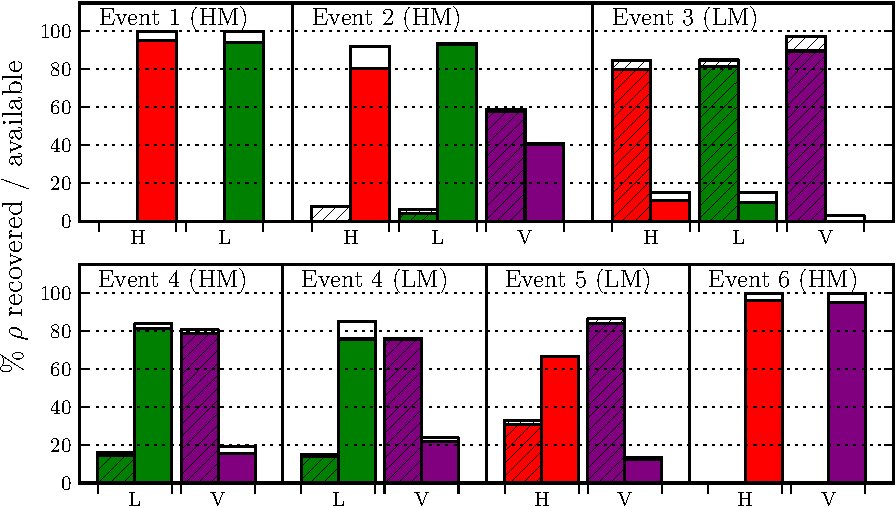
\includegraphics[width=\columnwidth]{papers/mdc2013_submission/figure5}}
%   \caption[SNR distribution]{\label{fig:snrDistribution}
% SNR recovered by \ihope{} as a fraction of total available SNR in each detector
% for each found injection. Hatched bars give the percentage of available SNR in
% the PN part of the injection; solid bars give the percentage of available SNR
% in the NR part. Color bars indicate the amount of SNR recovered by \ihope{}.
% ``LM" indicates events recovered by the low-mass search --- which used 3.5PN
% waveforms for templates --- ``HM" indicates events recovered by the high-mass
% search --- which used EOBNRv1 waveforms for templates. The PN SNR is determined
% by terminating the matched filter at the frequency half-way between the
% hybridization range; the NR part is given by filtering from that frequency and
% up.  Remarkably, both the low-mass and high-mass searches recovered most of the
% NR SNR despite the templates not having merger and ringdown (low mass) or not
% calibrated to the numerical waveforms used for the injections (high mass).
%   }
% \end{figure}

\section{Conclusion}
\label{sec:conclusions}

This chapter presents a systematic study to assess the ability to 
detect numerically modelled binary black hole data in real data taken from 
Initial LIGO and Virgo and recolored to predicted sensitivity curves of 
Advanced LIGO and Advanced Virgo in early observing runs. Building upon the 
work of the first NINJA project, this work, the culmination of the second NINJA 
project, studies the ability to do gravitational wave astronomy on a set of 60 
binary black hole hybrid waveforms submitted by 8 numerical relativity groups. 

In this work, a set of 7 numerically modelled binary black hole waveforms were 
added into the recolored data. This data was distributed to analysts with no 
knowledge of the parameters of the systems. 
% The unmodelled gravitational 
% waveform search pipeline, cWB, was able to recover one of these signals with an 
% estimated false alarm rate of 1 every 47 years. 
The matched-filtered compact 
binary merger search pipeline, \ihope{},
% using a bank of BBH IMR waveforms, 
% which were not calibrated against the NR signals used in NINJA-2,
was able 
to recover 6 of the waveforms with false alarm rate upper limits ranging 
between 
1 every 5800 years and 1 every 31000 years. 

% A range of parameter estimation codes were run on the 7 blind injections 
% that were added to the data used in this work. Though only results from
% the MCMC sampler were shown, these results proved to be statistically
% equivalent to estimates produce by the nested sampling and multinest
% samplers. These results demonstrate that it will be difficult to produce 
% precise estimate of black hole component masses and spins because of intrinsic 
% degeneracies between these parameters in the emitted waveforms. For some of the 
% BBH blind injections we find that a neutron-star--black-hole coalescence cannot 
% be ruled out. We also demonstrate the sensitivity of current parameter 
% estimation algorithms to non-Gaussian features in the data and explore the 
% ability to perform sky-localization of BBH observations.
% 
% A large-scale monte-carlo study was conducted to assess the efficiency of the 
% \ihope{} search pipeline as a function of the mass and angular momenta of the 
% component black holes. We find that for non-spinning equal mass waveforms the 
% sensitivity of the \ihope{} search pipeline in real noise, including 
% non-Gaussian artifacts, agrees well with predictions obtained using a 
% Gaussian-noise assumption. We have found evidence that adding waveform models 
% that include the effects of spin into the search pipeline will increase the 
% efficiency of binary black hole observation. We have also demonstrated that the 
% ability to recover numerical relativity waveforms, with identical parameters, 
% but submitted by different groups, is indistinguishable up to statistical 
% errors.

These results (completed by those in the published form~\cite{Aasi:2014tra})
represent the next step for the NINJA collaboration;
they address shortcomings in NINJA-1 while paving the way
for future work.  In a sense this work represents a baseline, as it
measures the ability of current gravitational-wave analyses to detect
and recover the parameters of an important subset of possible BBH
signals in non-Gaussian noise in the advanced detector era. 
From this baseline there are
multiple directions in which NINJA can expand. On the NR front,
groups are continuing to fill in the parameter space~\cite{Mroue:2013xna}.
As shown in
figure~\ref{fig:ParameterSpace}, even within the subspace of systems
with (anti-)aligned spins there are large regions left to explore.
Although NINJA-2 chose not to consider precessing signals many groups
already have or are working on such simulations~\cite{
Campanelli:2008nk, Tichy:2007hk, Tichy:2008du,Schmidt:2010it,
O'Shaughnessy:2011fx,Mroue:2012kv,O'Shaughnessy:2012vm,
O'Shaughnessy:2012ay,Hinder:2013oqa,Taracchini:2013rva}. Similarly, although 
the analyses used only the
$\ell=m=2$ mode in this work, it is expected that higher modes will be
important for detection and parameter
recovery~\cite{Pekowsky:2012sr,Healy:2013jza,McWilliams:2010eq,Brown:2012nn,
Pan:2011gk}.  Additional modes have been provided for many of
the waveforms in the NR catalog, although they have not yet been
validated.  In all cases, as additional waveforms and modes become
available they can be injected into the noise allowing for systematic
tests of both detection and parameter estimation analyses.

In parallel the detection and parameter estimation analyses continue to 
evolve and improve. There is much development work ongoing to improve the 
analytical waveform models that are used in analysis pipelines, particularly 
for inspiral-merger-ringdown waveforms. It seems likely that before the 
first aLIGO and AdV observation runs generic fast IMR precessing analytic 
models will be 
available~\cite{Santamaria:2010yb,Taracchini:2012ig,Pan:2013rra,Hannam:2013oca,
Taracchini:2013rva}.
Improvements in how detection pipelines deal with non-Gaussianities are being 
explored to attempt to achieve the maximum possible sensitivity to BBH signals 
across the parameter space. A number of efforts are ongoing to implement 
aligned-spin waveform models into  search algorithms. 
% As we have demonstrated here, 
This will increase sensitivity to BBH systems with aLIGO and 
AdV~\cite{Brown:2012qf,Ajith:2012mn,Harry:2013tca}.
Work is also underway to develop more realistic models 
of detector noise for parameter estimation pipelines, which account for the 
non-stationarity and non-Gaussianity present in real 
noise~\cite{Littenberg:2013gja}.  Accounting for such features
is expected to greatly reduce systematic biases in the recovered masses and 
spins.%, such as those seen in event 1.
The results presented here (completed by those published in~\cite{Aasi:2014tra})
can provide a measure against which these
next-generation analyses can be compared, in a way that measures not only their
response to signals but also to realistic noise.

